\documentclass{article}
\usepackage{NotesPackage}
\usepackage{csquotes}
\usetikzlibrary{arrows,decorations.pathmorphing}  % for photon squiggly arrows
\usepackage[section]{placeins}  % make all figures show before the start of the next section

\title{Modern Physics}
\date{September 16, 2019}
\author{Willoughby Seago}

\counterwithin{figure}{section}
\counterwithin{table}{section}
\counterwithin{equation}{section}

%\newcommand{\expected}[1]{\left\langle {#1} \right\rangle}
\newcommand{\braopket}[3]{\left\langle{#1}\middle|{#2}\middle|{#3}\right\rangle}
%\newcommand{\inlinedv}[3][]{\mathrm{d}^{#1}{#2}/\mathrm{d}{#3}^{#1}}
%\newcommand{\inlinepdv}[3][]{\partial^{#1}{#2}/\partial{#3}^{#1}}
%\newcommand{\dvat}[4][]{\dv[#1]{#2}{#3}\Biggr|_{#4}}

% counter for the decimal place of the equation number
\newcounter{equationDecimal}[section]

% get the equation number in the form <section number>.<equation number> and increment the equation counter
\newcommand{\eqNum}{\addtocounter{equationDecimal}{1}\thesection.\theequationDecimal}

\newcommand{\notesVersion}{1.0}
\newcommand{\notesDate}{04/01/2021}

\begin{document}
    \maketitle
    These are my notes for the \textit{modern physics} course from the University of Edinburgh as part of the second year of the theoretical physics degree.
    When I took this course in the 2019/20 academic year it was taught by Professor Alex Murphy\footnote{\url{https://www.ph.ed.ac.uk/people/alex-murphy}} and Professor Judy Hardy\footnote{\url{https://www.ph.ed.ac.uk/people/judy-hardy}}.
    These notes are based on the lectures delivered as part of this course, and the notes provided as part of this course.
    The content within is correct to the best of my knowledge but if you find a mistake or just disagree with something or think it could be improved please let me know.
    
    These notes were produced using \LaTeX\footnote{\url{https://www.latex-project.org/}}.
    Graphs where plotted using Python\footnote{\url{https://www.python.org/}}, Matplotlib\footnote{\url{https://matplotlib.org/}}, NumPy\footnote{\url{https://numpy.org/}}, and SciPy\footnote{\url{https://scipy.org/scipylib/}}.
    Diagrams were drawn with tikz\footnote{\url{https://www.ctan.org/pkg/pgf}}.
    Some images were taken from the lecture notes provided.
    
    This is version \notesVersion~of these notes, which is up to date as of \notesDate.
    \begin{flushright}
        Willoughby Seago
        
        s1824487@ed.ac.uk
    \end{flushright}
    \clearpage
    \tableofcontents
    \listoffigures
    \listoftables
    \clearpage
    
    \part{Special Relativity}
    \section{Relativity}
    A frame of reference has a time and a place, one description is:
    \begin{displayquote}
        A frame of reference is an array of rigid, massless, interpenetrable rods defining a grid over space
    \end{displayquote}
    In other words it is a coordinate system for time and space. We describe space with vectors relative to some origin point.
    The unit vectors \(\vi\), \(\vj\) and \(\vh k\) are used in 3D or more generally unit vectors \(\ve i\).
    A position vector \(\vv r\) is given as:
    \[\vv r = x \vi + y \vj + z \vh k\]
    or in more dimensions using Einstein summation convention:
    \[\vv r = r_i\ve i\]
    where \(r_i = \vv r\cdot\ve i\)
    Velocity is the rate of change of position and is given as:
    \[\dv{\vv r(t)}{t} = \dv{t}x(t)\vi + \dv{t}y(t)\vj + \dv{t}z(t)\vh k\]
    In more dimensions
    \[\dv{\vv r(t)}{t} = \dv{t}r_i(t) \ve i\]
    Note that this is only true in Cartesian coordinates:
    \[\dv{\vv r(t)}{t} = \dv{t}(r_i(t)\ve i) = \dv{r(t)}{t}\ve i + \dv{\ve i}{t}r(t) = \dv{r(t)}{t}\ve i  + 0\]
    This follows from the fact that the Cartesian unit vectors are necessarily invariant in time.
    Alternative notation that is used is \(\dot x\) or \(v_x\) for \(\mathrm{d}x/\mathrm{d}t\).
    
    Acceleration is the rate of change of velocity and is given as:
    \begin{align*}
        \dv[2]{\vv r(t)}{t} &= \dv[2]{t}x(t)\vi + \dv[2]{t}y(t)\vj + \dv[2]{t}z(t)\vh k\\
        &= \dot v_x\vi + \dot v_y\vj + \dot v_z\vh k\\
        &= a_x\vi + a_y\vj + a_z\vh k
    \end{align*}
    Or in more dimensions:
    \begin{align*}
        \dv[2]{\vv r(t)}{t} &= \dv[2]{r_i}{t}\ve i\\
        &= \dv{v_i}{t}\ve i\\
        &= a_i\ve i
    \end{align*}
    Again this only works in Cartesian coordinates
    
    For the time element of the reference frame in Cartesian/Galilean space one can think of a ``master clock" which can be read instantaneously from anywhere and is the only true measure of time.
    
    Relativity is about comparing measurements made in different reference frames. Galilean relativity is valid for all speeds \(v\ll c\) where as Einstein's relativity is valid for all speeds \(v\) in an inertial frame (special relativity) or not (general relativity)
    
    \section{Galilean Relativity}
    \subsection{Inertial Frames}
    Newton's first law:
    \begin{displayquote}
        In an inertial frame of reference an isolated particle moves at constant velocity
    \end{displayquote}
    This law can instead be used to define an inertial frame
    
    Suppose we have an inertial frame of reference \(S\), a second frame of reference \(S'\) and a particle \(P\).
    \begin{center}
        \begin{tikzpicture}
            % \draw[lightgray] (0, 0) grid (5, 5);
            \draw[->] (0, 0) -- (1, 0);d
            \draw[->] (0, 0) -- (0, 1);
            \draw[->] (0, 0) -- (0.7, 0.5);
            
            \node[right] at (1, 0) {\(\vh i\)};
            \node[above] at (0, 1) {\(\vh k\)};
            \node[above right] at (0.7, 0.5) {\(\vh j\)};
            \node[below left] at (0, 0) {\(S\)};
            
            \begin{scope}[xshift=3cm, yshift=4cm]
                \draw[->] (0, 0) -- (1, 0);
                \draw[->] (0, 0) -- (0, 1);
                \draw[->] (0, 0) -- (0.7, 0.5);
                
                \node[right] at (1, 0) {\(\vi'\)};
                \node[above] at (0, 1) {\(\vh k'\)};
                \node[above right] at (0.7, 0.5) {\(\vj'\)};
                \node[left] at (0, 0.5) {\(S'\)};
            \end{scope}
            
            \draw[->] (0, 0) -- (3, 4);
            \node at (2, 3) {\(\vv R\)};
            
            \draw[fill=black] (3, 1) circle (0.1cm);
            \node[below right] at (3, 1) {\(P\)};
            
            \draw[->] (0, 0) -- (2.9, 0.95);
            \node at (2, 0.5) {\(\vv r\)};
            
            \draw[->] (3, 4) -- (3, 1.1);
            \node[right] at (3, 2.5) {\(\vv r'\)};
        \end{tikzpicture}
    \end{center}
    The position vector of \(P\) can be given as \(\vv r\) or \(\vv r'\) with respect to \(S\) and \(S'\) respectively.
    It can be seen from the diagram that:
    \[\vv r = \vv R + \vv r'\tag{\eqNum}\]\label{eq:r=R+r'}
    If \(\dot{\vv R}\) is constant (ie \(S'\) is moving relative to \(S\) at a constant velocity) then \(\dot{\vv r}\) and \(\dot{\vv r}'\) are constant so \(S'\) must be an inertial frame. This is summed up as
    \begin{displayquote}
        A frame moving at a constant velocity relative to an inertial frame is itself an inertial frame
    \end{displayquote}

    \subsection{The `Standard Configuration'}
    To make solving problems involving two frames of reference easier there is a common way to set up the problem called the standard configuration
    The frames are set up such that all \(\ve i\) points in the same direction as \(\ve i'\), 
    \(S'\) moves at velocity \(\vv v\) relative to \(S\) (if possible \(\vv v\) only has a non-zero \(x\) component) 
    and the origin of \(S'\) is at the origin of \(S\) at time \(t = 0\).
    If two frames move with constant relative velocity \(\vv v\) then \(\vv R\), the vector connecting similar points, such as the origins of the two frames,
    is given by 
    \[\vv R = \vv v t\tag{\eqNum}\]\label{eq:R=vt}
    
    \subsection{Galilean Transformations}
    Galilean position transformation:
    
    This can be derived from equation~\ref{eq:r=R+r'} and equation~\ref{eq:R=vt}:
    \begin{align*}
        \vv r &= \vv R + \vv r'\\
        \vv r' &= \vv r - \vv R\\
        \vv R &= \vv v t\\
        \vv r' &= \vv r - \vv v t\\
    \end{align*}
    
    Galilean time transformation:
    
    This is simple since in Galilean relativity there is only one time:
    \[t=t'\]
    
    Galilean velocity transformation:
    
    This can be derived by differentiating equation~\ref{eq:r=R+r'} with respect to time:
    \[\dv{t}\vv r' = \dv{t}(\vv r-\vv R)\]
    If we call the velocity relative to frames \(S\) and \(S'\) \(\vv u\) and \(\vv u'\) respectively and as previously defined \(\dot{\vv R}=\vv v\) then we get:
    \[\vv u' = \vv u - \vv v\tag{\eqNum}\]\label{eq:u'=u-v}
    
    Galilean acceleration transformation:
    
    Since these are inertial frames the acceleration should be the same relative to either. We can show this by differentiating equation~\ref{eq:u'=u-v}
    \begin{align*}
        \dv{t}\vv u &= \dv{t}(\vv u-\vv v)\\
        \dv{\vv u'}{t} &= \dv{\vv u}{t} - \underbrace{\dv{\vv v}{t}}_{=0}\\
        \dv{\vv u'}{t} &= \dv{\vv u}{t}\\
        \vv a' &= \vv a
    \end{align*}
    
    In the standard configuration we can calculate for \(x\), \(y\) and \(z\) coordinates these transformations:
    \begin{center}
        \begin{tabular}{lrclrclrcl}
            Position: & \(x'\) & \hspace{-0.3cm}\(=\)\hspace{-0.3cm} & \(x-vt\) & 
            \(y'\) & \hspace{-0.3cm}\(=\)\hspace{-0.3cm} & \(y\) & 
            \(z'\) & \hspace{-0.3cm}\(=\)\hspace{-0.3cm} & \(z\)\\
            Velocity: & \(u_x'\) & \hspace{-0.3cm}\(=\)\hspace{-0.3cm} & \(u_x-v_x\) & 
            \(u_y'\) & \hspace{-0.3cm}\(=\)\hspace{-0.3cm} & \(u_y\) & 
            \(u_z'\) & \hspace{-0.3cm}\(=\)\hspace{-0.3cm} & \(u_z\)
        \end{tabular}
    \end{center}

    \section{19\(^\text{th}\) Century Relativity}
    In the \(19^\text{th}\) century people thought that all waves travelled in a medium and since light had wave-like properties it was a wave and therefore had a medium. Since light can travel in a vacuum this medium must fill the vacuum. The called this medium the luminiferous ether.
    
    The existence of this ether was shown to be false in the Michelson-Morley experiment.
    
    \begin{figure}[ht]
        \centering
        \begin{tikzpicture}
            %\draw[lightgray] (0, 0) grid (4, 4);
            \draw (0, 2) -- (4, 2);
            \draw (2, 0) -- (2, 4);
            \draw[ultra thick] (1.5, 4) -- (2.5, 4);
            \draw[ultra thick] (4, 1.5) -- (4, 2.5);
            \draw[->] (0, 2) -- (1, 2);
            \draw[->] (2, 2) -- (2.5, 2);
            \draw[->] (4, 2) -- (3.5, 2);
            \draw[->] (2, 2) -- (2, 2.5);
            \draw[->] (2, 4) -- (2, 3.5);
            \draw[->] (2, 2) -- (2, 1);
            \draw[rotate around={45:(2,2)}] (1.5, 1.9) rectangle (2.5, 2.1);
            \node[above] at (2, 4) {Mirror 1};
            \node[right] at (4, 2) {Mirror 2};
            \node[above right] at (2.25, 2.25) {Mirror 3};
            \node[below] at (2, 0) {Telescope};
            \node[left] at (0, 2) {Light source};
        \end{tikzpicture}
        \caption{The set up of the Michelson-Morley experiment}
        \label{Michelson-Morley setup}
    \end{figure}
    The Michelson-Morley experiment is shown in figure~\ref{Michelson-Morley setup}. 
    It consists of a semi-silvered mirror (mirror 3) and two normal mirrors (mirrors 1 and 2).
    Coherent light from the light source is split by the semi-silvered mirror. 
    Half of the light goes on to reflect off mirror 1 and the other half reflects off of mirror 2. 
    It then recombines and goes into the telescope.
    
    In the telescope fringes are seen if the difference between the path lengths of the two paths is not a multiple of the wavelength.
    
    The theory is that since the earth is moving (relative to the sun) it is probably moving through the ether. 
    Therefore the light in the experiment will either be travelling with (and then against after reflection) the ether in one direction or across the ether in the other direction.
    
    The entire setup is then rotated through a right angle. 
    This means that the path going with the ether swaps with the path going across the ether. 
    This should result in a change in the fringe pattern but it doesn't.
    This means that there isn't an ether and that the speed of light is constant.
    
    \section{Postulates of Special Relativity}
    
    A Van de Graff accelerator can be used to create a burst of electrons.
    The velocity of these electrons can be measured by timing how long they take to travel a certain distance.
    It is possible  use them to induce a current in a circuit to trigger a timer to do this.
    We can also measure their kinetic energy \(T\) by absorbing them and  measuring the temperature change.
    Classically we would expect
    \[T=\frac{1}{2}mv^2\implies v\propto \sqrt{T}\]
    
    \begin{figure}[ht]
        \centering
        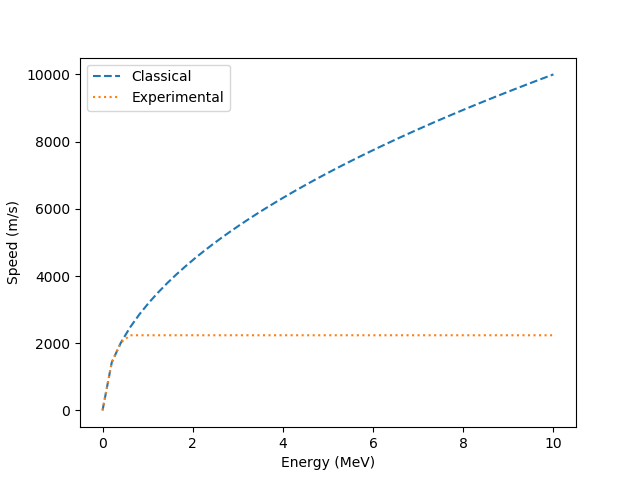
\includegraphics[scale=0.8]{classical_vs_experimental_electron_speed.png}
        \caption{A graph of speeds of electrons as predicted classically and measured experimentally}
        \label{fig:classical vs experimental electron speeds}
    \end{figure}

    It can be seen in figure~\ref{fig:classical vs experimental electron speeds} that the experimental results flatten out. 
    This happens around \(\SI{0.5}{MeV}\) which is the rest mass of an electron.
    In all cases \(c\) is observed as the 'limiting speed'.
    
    \subsection{The Postulates}
    The postulates of special relativity are:
    \begin{enumerate}
        \item Special relativity postulate 1 (SR1) - The laws of physics are the same in all inertial frames.
        \item Special relativity postulate 2 (SR2) - The speed of light in a vacuum is constant in all inertial frames.
    \end{enumerate}

    SR1 implies that all inertial frames are equivalent and that only relative motion within a frame is important.
    SR1 and SR2 combined imply that \(c\) is the ultimate speed limit regardless of frame of reference.
    
    \(c\) is defined as \(\SI{2.99792458e6}{m.s^{-1}}\) (note that the units are included in \(c\)).
    
    \(\SI{1}{m}\) is defined as the distance travelled by light in a vacuum in \(1/c\,\si{s}\).
    
    (\(\SI{1}{s}\) is defined by radioactive decay rates so there is some intrinsic uncertainty)
    
    \subsection{Traverse Stick}
    Two rods \(A\) and \(B\) of length \SI{1}{m} each are parallel. One of them is moving at speed \(v\approx c\) relative to the other. From the perspective of \(A\) does \(B\) change length?
    
    No. Both rods stay the same length. We can show this using SR1. If from \(A\)'s point of view \(B\)'s length changes by some amount \(\Delta L\) then from \(B\)'s frame of reference \(A\)'s length must also increase by \(\Delta L\) both rods are in inertial frames moving relative to each other. This means since \(A\)'s length doesn't change in its reference frame it also can't change in \(B\)'s reference frame.
    
    \subsection{The Observer}
    An observer in relativity theory is an intelligent experimentalist. Intelligent means that they interpret data in accordance with SR1 and SR2. Experimentalist means that the take and collate measurements.
    
    In Galilean geometry there was a universal time. Finite \(c\) renders this problematic. In special relativity we again need a rigid, massless array of interpenetrable rods defining a grid over space but we also need an array of synchronised clocks at the grid points.
    
    \section{Lorentz Factor}
    \subsection{Terminology}
    An event is where \emph{and} when something happened. 
    Relativity deals with the relationship between the coordinates of events. 
    Coordinates are given as four-vectors \((x, y, z, t)\) which are vectors with three space components and one time component. 
    To make things simpler we often limit ourselves to \((x, t)\).
    Due to relativity it only makes sense to quote time and place together.
    
    Two events are simultaneous if they have the same time coordinate
    
    The time interval between two events with the same spatial coordinates is known as the proper time and is denoted \(\tau_0\). All other time intervals are improper and are denoted \(\tau\).
    
    A clock is something that generates regular events.
    
    \subsection{Moving Clocks Run Slowly}
    Imagine a clock and an observer. 
    If both clock and observer are at rest in a given inertial frame then the time between ticks of the clock is a proper time \(\tau_0\). 
    If instead both the clock and the observer are both moving at a constant velocity then they are stationary in their own reference frame so the time between ticks is still \(\tau_0\).
    However if the clock is moving at a constant speed relative to the observer then the observer will measure improper time \(\tau\) between ticks where \(\tau>\tau_0\).
    
    \subsection{Lorentz Factor Derivation}
    A clock can be constructed from two mirrors. 
    A photon is emitted at one mirror, reflects off the other and then arrives at the first mirror and the clock has ticked once.
    
    \begin{figure}[ht]
        \centering
        \begin{tikzpicture}[
        >=stealth',
        pos=.8,
        photon/.style={decorate,decoration={snake,post length=1mm}}
        ]
            %\draw[lightgray] (0, 0) grid (10, 5);
            
            % Frame S'
            \draw[ultra thick] (1, 0) -- (2, 0);
            \draw[ultra thick] (1, 5) -- (2, 5);
            \draw[->, photon] (1.5, 0) -- (1.5, 2);
            \draw[<->] (0.5, 0) -- (0.5, 5);
            \node[left] at (0.5, 2.5) {\(l_0\)};
            \node[below] at (1.5, 0) {Frame \(S'\)};
            
            % Seperator
            \draw[dashed, lightgray] (2.5, -1) -- (2.5, 6);
            
            % Frame S
            \draw[ultra thick] (3, 0) -- (4, 0);
            \draw[ultra thick] (3, 5) -- (4, 5);
            \draw[ultra thick] (6, 0) -- (7, 0);
            \draw[ultra thick] (6, 5) -- (7, 5);
            \draw[ultra thick] (9, 0) -- (10, 0);
            \draw[ultra thick] (9, 5) -- (10, 5);
            \draw[->, photon, rotate around={-31:(3.5, 0)}] (3.5, 0) -- (3.5, 2);
            \draw[->, photon, rotate around={31:(6.5, 5)}] (6.5, 5) -- (6.5, 3);
            \draw (3.5, 0) -- (6.5, 5);
            \draw (6.5, 5) -- (9.5, 0);
            \draw[<->] (3.5, 5.5) -- (6.5, 5.5);
            \node[above] at (5, 5.5) {\(v\tau/2\)};
            \node[below] at (6.5, 0) {Frame \(S\)};
            \draw[->] (4.1, 0) -- (5, 0) node[right] {\(v\)};
            \node[above left] at(5, 2.5) {\(L\)};
        \end{tikzpicture}
        \caption{Mirror-photon clock}
        \label{fig:mirror-photon clock}
    \end{figure}

    The diagram in figure \ref{fig:mirror-photon clock} shows the same setup in two reference frames. 
    Frame \(S'\) is stationary and frame \(S\) is an inertial frame moving at constant speed relative to frame \(S\).
    
    There are three events that occur in both frames:
    \begin{enumerate}
        \item A photon is emitted
        \item The photon reflects off of the upper mirror
        \item The photon arrives back at the first mirror
    \end{enumerate}
    We can work out the coordinates of these events in both frames. 
    They are given in tables \ref{tab:events in frame S'} and \ref{tab:events in frame S}.
    
    \begin{table}[ht]
        \centering
        \begin{tabular}{c|ccc}
            Event & \(x\) & \(y\) & t\\ \hline
            1 & 0 & 0 & 0\\
            2 & 0 & \(l_0\) & \(l_0/c\)\\
            3 & 0 & 0 & \(2l_0/c\)
        \end{tabular}
        \caption{Events in frame \(S'\)}
        \label{tab:events in frame S'}
        \vspace{0.5cm}
        \begin{tabular}{c|ccc}
            Event & \(x\) & \(y\) & t\\ \hline
            1 & 0 & 0 & 0\\
            2 & \(v\tau/2\) & \(l_0\) & \(L/c\)\\
            3 & \(2v\tau/2\) & 0 & \(2L/c\)
        \end{tabular}
        \caption{Events in frame \(S\)}
        \label{tab:events in frame S}
    \end{table}
    
    What is the time interval \(\Delta t_{13}' = \tau_0\)?
    \[\Delta t_{13}' = \frac{2l_0}{c}\]
    What is the time interval \(\Delta t_{13} = \tau\)?
    \[\Delta t_{13} = \frac{2L}{c}\]
    Note that this is an improper time as the \(x\) coordinates of events 1 and 3 are different in frame \(S\).
    
    From the diagram in figure \ref{fig:mirror-photon clock} we can see that
    \begin{align*}
        L^2 &= l_0^2 + \left(\frac{v\tau}{2}\right)^2\\
        \left(\frac{c\tau}{2}\right)^2 &= l_0^2 + \left(\frac{v\tau}{2}\right)^2\\
        \frac{c^2\tau^2}{4} &= l_0^2 + \frac{v^2\tau^2}{4}\\
        c^2\tau^2 &= 4l_0^2 + v^2\tau^2\\
        4l_0^2 &= (c^2 - v^2)\tau^2\\
        \tau^2 &= \frac{4l_0^2}{c^2-v^2}\\
        \tau &= \frac{2l_0}{\sqrt{c^2-v^2}}\\
        \tau &= \frac{2l_0}{c\sqrt{1 - v^2/c^2}}
        \intertext{Substitute in \(\tau_0 = 2l_0/c\)}
        \tau &= \frac{1}{\sqrt{1-v^2/c^2}}\tau_0\\
        \tau &= \gamma\tau_0
    \end{align*}
    This is time dilation.
    \(\gamma = (1-v^2/c^2)^{-1/2}\) is the Lorentz factor.
    Since \(v \le c\) and \(v^2>0\) we can see \(\gamma\ge 1\A v\).
    As \(v\to 0\) \(\gamma\to 1\) therefore \(\tau\to\tau_0\).
    This shows that classical physics still works for sufficiently small \(v\).
    For \(v\ll c\) we can use the binomial expansion of \((1 + x)^n\approx 1 + nx\) where \((|x|<1)\)
    \[\gamma = \left(1 - \frac{v^2}{c^2}\right)^{-\frac{1}{2}}\]
    \[\gamma \approx 1 + \frac{1}{2}\frac{v^2}{c^2}\]
    This approximation also helps support the fact that this agrees with classical physics.
    
    \begin{figure}[ht]
        \centering
        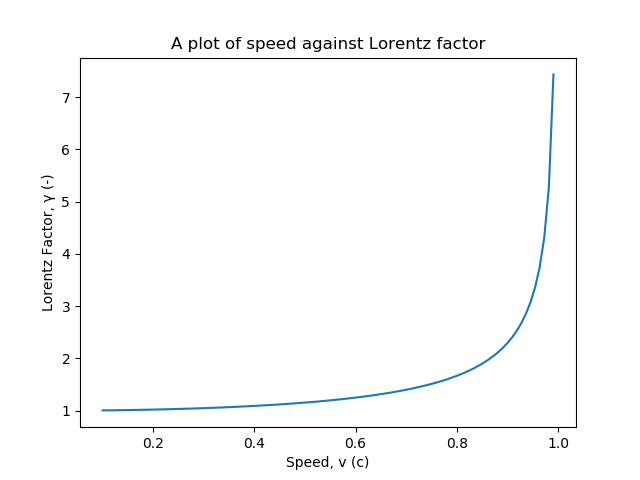
\includegraphics[scale=0.8]{speed_vs_Lorentz_factor.png}
        \caption{A graph showing the values \(\gamma\) takes}
    \end{figure}

    \subsection{Decay Review}
    One of the classic experiments to support this time dilation is related to the decay of muons.
    To understand it we should recap nuclear decay.
    
    Consider a collection of \(N_0\) things at time \(t=0\). 
    Each thing has an independent chance of doing a specific thing in a set period. 
    For example imagine 100 plates each of which has a \SI{20}{\%} chance of breaking within a year. 
    We can write a function \(N(t)\) to describe the number of plates left after \(t\) years.
    After 1 year \SI{20}{\%} of the plates have smashed:
    \[N(1) = 0.8N_0\]
    After 20 years there are
    \[N(20) = 0.8^{20}N_0\]
    In general for a starting number of \(N\) things with a probability \(p\) of the thing in question occurring after time \(t\) there are
    \[N(t) = N_0p^t\]
    left where the thing hasn't happened.
    We can work out the half life by setting \(N(t) = N_0/2\):
    \begin{align*}
        \frac{N_0}{2} &= N_0p^{t_{1/2}}\\
        \frac{1}{2} &= p^{t_{1/2}}\\
        \ln\frac{1}{2} &= t_{1/2}\ln p\\
        \frac{\ln(1/2)}{\ln p} &= t_{1/2}
    \end{align*}
    This equation also follows from the rate of decay equation
    \begin{align*}
        -\dv{N}{t} &\propto N\\
        -\dv{N}{t} &= \lambda N\\
        \frac{1}{N}\dv{N}{t} &= -\lambda\\
        \int_{N_0}^{N}\frac{1}{N}\dv{N}{t}\,dt &= -\lambda\int_{t_0}^{t}\,dt\\
        \int_{N_0}^{N}\frac{dN}{N} &= -\lambda\int_{t_0}^{t}\,dt\\
        [\ln N]_{N_0}^N &= -\lambda[t]_{t_0}^t\\
        \ln N - \ln N_0 = -\lambda(t - t_0)
        \intertext{\(t_0 = 0\)}
        \ln\frac{N}{N_0} &= -\lambda t\\
        \frac{N}{N_0} &= e^{-\lambda t}\\
        N &= N_0e^{-\lambda t}
    \end{align*}
    At time \(t = \tau = 1/\lambda\) \(N = N_0e^{-1} \approx 0.37 N_0\)
    We call this the characteristic decay time \(\tau\). It corresponds to \(1/e\) of the sample being left.
    We also have the relationship
    \[t_{1/2} = \tau \ln 2\]
    This is important in the experiment with muon decay times.
    
    \section{Experimental Evidence and Length Contraction}
    \subsection{Muon Decay Evidence}
    We can compare the number of muons at the top of a mountain and at sea level. 
    We select muons with speed \(v = 0.995c\) which means they have a Lorentz factor of \(\gamma \approx 10\). 
    The lifetime of a muon in its own frame is \(\SI{2.2}{\mu s}\). 
    If the height of the mountain is \(l_0\) then classical physics would predict the time taken to reach the base of the mountain is 
    \[t = \frac{l_0}{0.995c} = \SI{6.39}{\mu s}\]
    This means we would expect a fraction \(P\) of the muons to reach the base:
    \[P = e^{-t/\tau} = e^{-6.39/2.2}\approx 0.05\]
    However when we actually do this experiment we find that \(P = 0.72\pm 0.03\ne 0.05\).
    
    We can explain this inconsistency using special relativity.
    In the lab frame 
    \[\tau = \gamma\tau_0 = \SI{22}{\micro s}\implies P = e^{-6.39/22}\approx 0.75\]
    This matches up with the experimental result.
    
    However in relativity we need to be able to explain effects like this from both frames involved, so what is happening in the muons frame? 
    There can't be any time dilation as the muons lifetime is defined in its frame.
    The answer is that from the muons frame an observer sees length contraction of the distance the muon must travel.
    The improper length \(l\) can be calculated as
    \begin{equation}\label{eqn:length contraction}
        l = \frac{l_0}{\gamma}
    \end{equation}
    The derivation of equation \ref{eqn:length contraction} can be found in the next section
    
    \subsection{Length Contraction Derivation}
    Consider a train moving along a track relative to a platform. What is the length of the platform as viewed from:
    \begin{itemize}
        \item The platform
        \item The train
    \end{itemize}
    An observer on the platform can measure its proper length. 
    To do this they flash a light at the centre of the platform. 
    This generates simultaneous measurements at either end. 
    If it takes time \(T\) for the light to travel from its source to the edge of the platform then the length of the platform is \(l_0 = 2cT\). 
    There are two important events \((x, t)\).
    They are when the light reaches either end of the platform: \((0, T)\) and \((2cT, T)\). Since both have \((t = T)\) any length measured is proper.
    
    The train now travels at speed \(v\) parallel to the platform. 
    It rapidly flashes a light so that the light flashes at either end of the platform.
    In the platform's frame there is an event \((0, t_1)\) when the train passes a clock at one end of the platform.
    There is a second event \((l_0, t_2)\) when the train passes the far end of the platform.
    The time interval is \(\Delta t = \tau = t_2 - t_1\).
    This is an improper time since the events occur in different locations.
    The observer can confirm that \(l_0 = v\tau\).
    
    In the train's frame of reference an observer sees the platform go past at speed \(v\). 
    The events \((x', t')\) corresponding to passing either end of the platform are: \((0, t_1')\) and \((0, t_2')\). 
    The time difference between these is \(\Delta t' = \tau_0 = t_2' - t_1'\).
    Note that this is a proper time since the observer is stationary in the train's frame of reference.
    The observer can then deduce that the length of the platform is \(\Delta x' = l = v\tau_0\).
    This is an improper length since the positions of the ends of the platform were taken at two different times.
    
    We can compare the ratios of the lengths measured by the observers to get
    \[\frac{l}{l_0} = \frac{v\tau_0}{v\tau} = \frac{\tau_0}{\tau} = \frac{\tau_0}{\tau_0\gamma} = \frac{1}{\gamma}\]
    \[l = \frac{l_0}{\gamma}\]
    
    \subsection{Space-time}
    Time dilation from one frame is seen as length contraction in another. 
    This means that they are the same effect. Space and time are `enmeshed' with one another in a way that doesn't occur in Newtonian/Galilean physics.
    
    \subsection{Twin's Paradox}
    If you where to travel to the nearest start \(\Gamma\)-Centauri which is \SI{4}{ly} away and you travel at speed \(0.8c\) and, upon arriving, immediately start the return trip how much time has elapsed on Earth when you return?
    
    From an observer on Earth distance to the star is a proper length as the distance isn't changing (by a meaningful amount since we are talking light year distances). 
    This means that in Earth's frame of reference times are all measured at the same location, therefore the time taken is
    \[\frac{4}{0.8}\cdot 2 = \SI{10}{yrs}\]
    How much time has passed from your point of view?
    
    An observer on board the ship sees the clock moving with the ship so it measures a proper time. 
    Earth is moving away and then back again so time duration \(t_E\) on Earth, as observed from the ship, is an improper time and hence is bigger than the proper time \(t_0\) measured on the ship by a factor of \(\gamma\).
    \[t_E = t_0\gamma\implies t_0 = \frac{t_E}{\gamma} = 10\sqrt{1-0.8^2} = \SI{6}{yrs}\]
    But the system is symmetric so how does one observer age less than the other? 
    Special relativity isn't enough, the ship must accelerate at least to turn around half way and also to get up to speed. 
    This means we need to use general relativity.
    
    \subsection{Synchronised Clocks}
    To synchronise two clocks we flash a light halfway between them and use the light reaching them as a simultaneous event to set the clocks by.
    What if the frame of the clocks moves relative to another observer?
    This is shown in figure \ref{fig:synchronising moving clocks}.
    An important factor is that the light still moves at speed \(c\) in both frames.
    \begin{figure}[ht]
        \centering
        \begin{tikzpicture}[
        >=stealth',
        pos=.8,
        photon/.style={decorate,decoration={snake,post length=1mm}}
        ]
            %\draw[lightgray] (0, 0) grid (10, 6);
            \draw[|-|] (0, 5) -- (5, 5);
            \node[below] at (0, 5) {\(A\)};
            \node[below] at (5, 5) {\(B\)};
            \node[below] at (2.5, 5) {\(M\)};
            
            \begin{scope}[xshift=2cm, yshift=-2cm]
                \draw[|-|] (0, 5) -- (5, 5);
                \node[below] at (0, 5) {\(A\)};
                \node[below] at (5, 5) {\(B\)};
                \node[below] at (2.5, 5) {\(M\)};
            \end{scope}
            
            \begin{scope}[xshift=4cm, yshift=-4cm]
                \draw[|-|] (0, 5) -- (5, 5);
                \node[below] at (0, 5) {\(A\)};
                \node[below] at (5, 5) {\(B\)};
                \node[below] at (2.5, 5) {\(M\)};
            \end{scope}
            
            \node at (10, 5) {\(t = 0\)};
            \node at (10, 3) {\(t = t_A\)};
            \node at (10, 1) {\(t = t_B\)};
            
            \draw[gray, dashed] (0, 4.5) -- (0, 0);
            \draw[gray, dashed] (2, 2.5) -- (2, 2);
            \draw[gray, dashed] (4, 0.5) -- (4, 0);
            
            \draw[<->] (0, 2) -- (2, 2);
            \draw[<->] (0, 0) -- (4, 0);
            
            \node[below] at (1, 2) {\(vt_A\)};
            \node[below] at (2, 0) {\(vt_B\)};
            
            \draw[photon, ->] (2.5, 5.5) -- (3.5, 5.5);
            \draw[photon, ->] (2.5, 5.5) -- (1.5, 5.5);
            
            \draw[photon, ->] (3, 3.5) -- (2, 3.5);
            \draw[photon, ->] (5, 3.5) -- (6, 3.5);
            
            \draw[photon, ->] (8, 1.5) -- (9, 1.5);
            
            \draw[->] (7, 6) -- (8, 6) node[right] at (8, 6) {\(v\)};
            \draw[->] (7, 6) -- (7, 5) node[below] at (7, 5) {\(t\)};
        \end{tikzpicture}
        \caption{Clocks moving while they are synchronised}
        \label{fig:synchronising moving clocks}
    \end{figure}
    Viewed from the frame of reference of the page 
    \[AM = MB = \frac{l_0}{2\gamma}\]
    \[ct_A = \frac{l_0}{2\gamma} - vt_A\implies t_A = \frac{l_0}{2\gamma(c + v)}\]
    \[ct_B = \frac{l_0}{2\gamma} + vt_B\implies t_A = \frac{l_0}{2\gamma(c - v)}\]
    Crucially \(t_A\ne t_B\) so the clocks aren't synchronised.
    \(t_A < t_B\) this can be remembered with the mnemonic \textbf{l}eading clocks \textbf{l}ag.
    
    \subsection{Rod-Shed Paradox}
    A rod length \(l\) moves through a shed which has two doors opposite each other. 
    With the door closed the largest rod that can fit in the shed has length \(l\).
    If the rod moves towards and trough the shed from the shed we observe the rod's length contracting so it fits comfortably in the shed and we can close both doors for a short time.
    From the rod's frame of reference we observe the shed contracting so the rod won't fit so we can't close both doors at the same time.
    
    The solution is that in the frame of reference of the rod the two doors don't both close at the same time. Only one closes at a time.
    
    The reason that a rod moving parallel to its length contracts is that it has a leading edge.
    A rod moving perpendicular to its length has no leading edge so experiences no time dilation (assuming it has no width, if it does then the width contracts).
    Having a leading edge means that one edge lags in time so we can't measure both ends simultaneously so we can't measure proper length.
    
    \section{Lorentz Transformations and Minkowski Diagrams}
    \subsection{Lorentz Transformations}
    \[
        \begin{array}{cccc}
            x' = \gamma(x - vt) & y' = y & z' = z & t' = \gamma(t - vx/c^2)\\[0.25cm]
            \Delta x' = \gamma(\Delta x - v\Delta t) & \Delta y' = \Delta y & \Delta z' = \Delta z & \Delta t' = \gamma(\Delta t - v\Delta x/c^2)
        \end{array}
    \]
    In frame \(S'\) a clock, unmoving at the origin registers two events.
    The time interval between these events is \(\Delta t' = \tau_0\), a proper time since the clock is stationary.
    In frame \(S\), which is moving with respect to frame \(S'\), the time interval is \(\Delta t = \tau\), an improper time.
    \[\Delta x' = \gamma(\Delta x-v\Delta t) = 0\]
    \[\implies \Delta t = \frac{\Delta x}{v}\]
    \begin{align*}
        \tau_0 &= \Delta t'\\
        &= \gamma\left(\Delta t - \frac{v\Delta x}{c^2}\right)\\
        &= \gamma\left(\Delta t - \frac{v^2\Delta t}{c^2}\right)\\
        &= \gamma\Delta t\left(1 - \frac{v^2}{c^2}\right)\\
        &= \gamma\Delta t\gamma^{-2}\\
        &= \frac{\Delta t}{\gamma}\\
        &= \frac{\tau}{\gamma}        
    \end{align*}
    \[\implies \tau_0 \gamma = \tau\]
    Which is the result that we expect from time dilation.
    
    \subsection{Velocity Transformation}
    Two frames \(S\) and \(S'\) are moving at speed \(v\) relative to each other.
    A particle has speed \(u\) in frame \(S\) and speed \(u'\) in frame \(S\).
    To determine a velocity we need two events as given in table \ref{fig:lorentz velocity transform events}
    \begin{figure}[ht]
        \centering
        \begin{tabular}{c|cc}
            Frame & Event 1 & Event 2\\ \hline
            \(S\) & \((0, 0)\) & \((x, t)\) \\
            \(S'\) & \((0, 0)\) & \((x', t')\)
        \end{tabular}
        \caption{Two events and their coordinates in frames \(S\) and \(S'\)}
        \label{fig:lorentz velocity transform events}
    \end{figure}
    We can use the simple formula
    \[\text{speed} = \frac{\Delta\text{distance}}{\Delta\text{time}}\]
    to calculate and compare the speed of the particle in both frames.
    In frame \(S\):
    \[u = \frac{x - 0}{t - 0} = \frac{x}{t}\]
    In frame \(S'\):
    \[u' = \frac{x' - 0}{t' - 0} = \frac{\gamma(x - vt)}{\gamma(1 - vx/c^2)} = \frac{x/t - v}{1 - xv/tc^2} = \frac{u-v}{1-uv/c^2}\]
    This gives us the Lorentz velocity transformation:
    \[u' = \frac{u - v}{1 - \frac{uv}{c^2}}\]
    
    \subsection{Minkowski Diagrams}
    Minkowski diagrams, also known as space-time diagrams are a graphical representation of space-time.
    The typically have four axes \(x\), \(y\), \(z\) and \(t\) although we often restrain ourselves to just \(x\) and \(t\).
    The world line of a particle is its path in the diagram.
    Typically it is convenient to modify the \(t\) axis to a \(ct\) axis.
    This is useful because it makes the numbers used for all axes comparable and makes the time axis into a spatial axis.
    
    A photon has a world line that is at \(45^\circ\) to the \(x\) axis in a two dimensions. 
    Any world line that makes a smaller angle than this must belong to a particle that is travelling faster than the speed of light.
    
    \begin{figure}[ht]
        \centering
        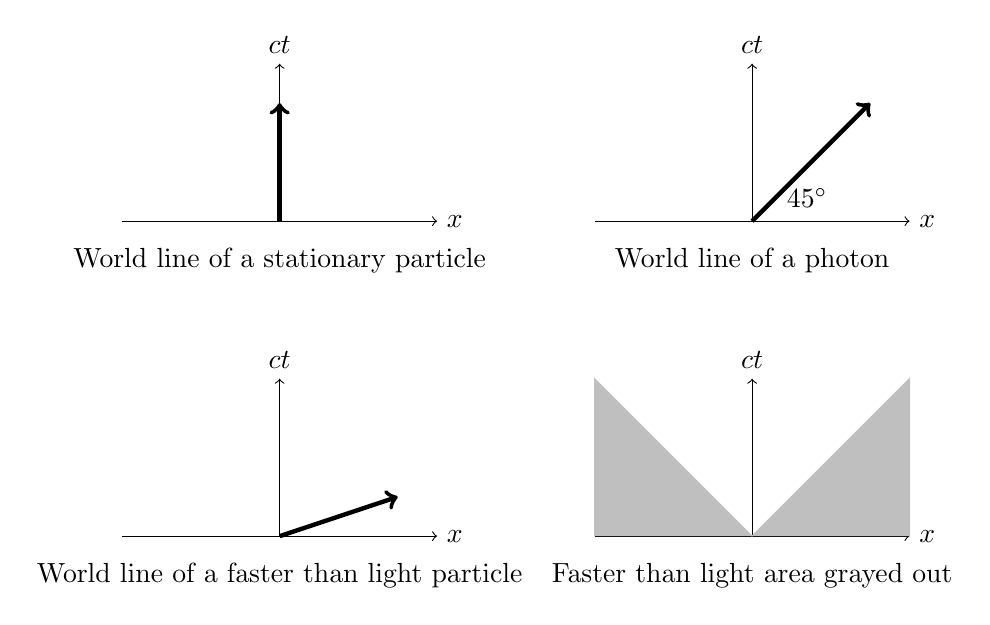
\begin{tikzpicture}
            %\draw[lightgray] (0, 0) grid (10, 10);
            
            \draw[->] (2, 7) -- (2, 9) node[above] at (2, 9) {\(ct\)};
            \draw[ultra thick, ->] (2, 7) -- (2, 8.5);
            \node at (2, 6.5) {World line of a stationary particle};
            
            \draw[->] (6, 7) -- (10, 7) node[right] at (10, 7) {\(x\)};
            \draw[->] (8, 7) -- (8, 9) node[above] at (8, 9) {\(ct\)};
            \draw[ultra thick, ->] (8, 7) -- (9.5, 8.5);
            \node at (8.7, 7.3) {\(45^\circ\)};
            \node at (8, 6.5) {World line of a photon};
            
            \draw[->] (0, 3) -- (4, 3) node[right] at (4, 3) {\(x\)};
            \draw[->] (2, 3) -- (2, 5) node[above] at (2, 5) {\(ct\)};
            \draw[ultra thick, ->] (2, 3) -- (3.5, 3.5);
            \node at (2, 2.5) {World line of a faster than light particle};
            
            \draw[->] (6, 3) -- (10, 3) node[right] at (10, 3) {\(x\)};
            \draw[->] (8, 3) -- (8, 5) node[above] at (8, 5) {\(ct\)};
            \draw[fill=lightgray, color=lightgray] (8, 3) -- (10, 5) -- (10, 3);
            \draw[fill=lightgray, color=lightgray] (8, 3) -- (6, 5) -- (6, 3);
            \node at (8, 2.5) {Faster than light area grayed out};
            \draw[->] (0, 7) -- (4, 7) node[right] at (4, 7) {\(x\)};
        \end{tikzpicture}
        \caption{World lines of faster than light particles}
    \end{figure}
    It is also possible to add multiple frames of reference in one diagram. 
    We do this by using the fact that the angle between a photon's world line and the axis must be the same for both the \(x\) and \(ct\) axes.
    This is shown in figure \ref{fig:two frames one minkowski diagram}
    \begin{figure}[ht]
        \centering
        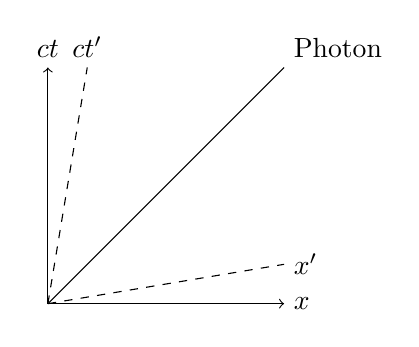
\begin{tikzpicture}
            %\draw[lightgray] (0, 0) grid (3, 3);
            \draw[->] (0, 0) -- (3, 0) node[right] at (3, 0) {\(x\)};
            \draw[->] (0, 0) -- (0, 3) node[above] at (0, 3) {\(ct\)};
            \draw (0, 0) -- (3, 3) node[above right] at (3, 3) {Photon};
            \draw[dashed] (0, 0) -- (0.5, 3) node[above] at (0.5, 3) {\(ct'\)};
            \draw[dashed] (0, 0) -- (3, 0.5) node[right] at (3, 0.5) {\(x'\)};
        \end{tikzpicture}
        \caption{Two reference frames shown on the same Minkowski diagram}
        \label{fig:two frames one minkowski diagram}
    \end{figure}
    It is possible to draw lines on the diagram where all events on the line are simultaneous. 
    This is done in figure \ref{fig:lines of simultaneity}. 
    Since these lines aren't parallel it can be seen that events that are simultaneous in one frame are not simultaneous in another.
    \begin{figure}[ht]
        \centering
        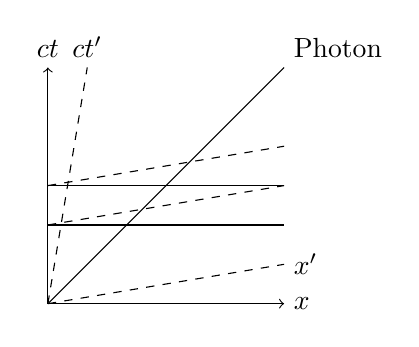
\begin{tikzpicture}
            %\draw[lightgray] (0, 0) grid (3, 3);
            \draw[->] (0, 0) -- (3, 0) node[right] at (3, 0) {\(x\)};
            \draw[->] (0, 0) -- (0, 3) node[above] at (0, 3) {\(ct\)};
            \draw (0, 0) -- (3, 3) node[above right] at (3, 3) {Photon};
            \draw[dashed] (0, 0) -- (0.5, 3) node[above] at (0.5, 3) {\(ct'\)};
            \draw[dashed] (0, 0) -- (3, 0.5) node[right] at (3, 0.5) {\(x'\)};
            \draw (0, 1) -- (3, 1);
            \draw (0, 1.5) -- (3, 1.5);
            \draw[dashed] (0, 1) -- (3, 1.5);
            \draw[dashed] (0, 1.5) -- (3, 2);
        \end{tikzpicture}
        \caption{Lines of simultaneity}
        \label{fig:lines of simultaneity}
    \end{figure}
    
    \section{Consequences of Special Relativity}
    \begin{figure}[ht]
        \centering
        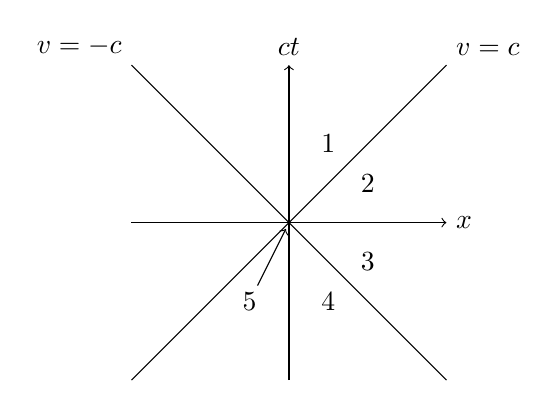
\begin{tikzpicture}
            \draw[->] (-2, 0) -- (2, 0) node[right] at (2, 0) {\(x\)};
            \draw[->] (0, -2) -- (0, 2) node[above] at (0, 2) {\(ct\)};
            \draw (-2, -2) -- (2, 2) node[above right] at (2, 2) {\(v=c\)};
            \draw (2, -2) -- (-2, 2) node[above left] at (-2, 2) {\(v=-c\)};
            \node at (0.5, 1) {1};
            \node at (1, 0.5) {2};
            \node at (1, -0.5) {3};
            \node at (0.5, -1) {4};
            \node at (-0.5, -1) {5};
            \draw[->] (-0.4, -0.8) -- (-0.04, -0.08);
        \end{tikzpicture}
        \caption{Regions of a Minkowski diagram}
        \label{fig:regions of a minkowski diagram}
    \end{figure}
    The regions shown on the diagram in figure \ref{fig:regions of a minkowski diagram} represent:
    \begin{enumerate}
        \item The future
        \item Faster than light travel to get into this region
        \item Things in this region don't have enough energy to influence now
        \item The past
        \item Now
    \end{enumerate}
    Together regions 1 and 4 make up the light cone of all places that something could be in the future or could have been in the past.
    Two things are causally disconnected until their light cones overlap.
    That is one can't affect the other when they don't have intersecting light cones.
    
    \subsection{Invariant Space-Time Interval}
    The invariant space-time interval is a property that is the same in all frames of reference.
    It is denoted \(s^2\) and in 2 dimensions \((x, ct)\) it has the value
    \[s^2 = (ct)^2 - x^2\]
    To show that this is invariant we start with it as measured from \(S'\) and use the Lorentz transforms:
    \[x' = \gamma(x - vt)\qquad \& \qquad t' = \gamma\left(t-\frac{vx}{c^2}\right)\]
    \begin{align*}
        s^2 &= (ct')^2 - x'^2\\
        &= \gamma^2\left(\left(ct-\frac{vx}{c}\right)^2 - (x-vt)^2\right)\\
        &= \gamma^2\left((c^2 - v^2)t^2 - \left(1-\frac{v^2}{c^2}\right)x^2\right)\\
        &= \gamma^2\left(c^2\left(1 - \frac{v^2}{c^2}\right)t^2 - \left(1-\frac{v^2}{c^2}\right)x^2\right)\\
        &= \gamma^2((ct)^2\gamma^{-2} - x^2\gamma^{-2})\\
        &= (ct)^2 - x^2
    \end{align*}
    This is trivial to extend into 4 dimensions as \(y=y'\) and \(z=z'\), this gives us
    \[s^2 = (ct)^2 - x^2 - z^2 - y^2\]
    
    \subsection{Relativistic Doppler}
    Classical Doppler:
    \[f_o = f_s\left(\frac{v\pm v_o}{v\pm v_s}\right)\]
    where \(o\) indicates value related to the observer, \(s\) indicates a value related to the source, \(v\) is the speed of the wave and \(f\) is a frequency.
    
    Consider the frame \(S\) in which the source is stationary at \((0, 0, 0, t)\). 
    If the wavelength is \(\lambda\) and the wave's speed is \(c\). 
    An observer is receding from the source at speed \(v\). 
    If one wave front has just reached the observer then the time until the next one is given by
    \[\Delta t = \frac{\lambda}{c - v}\]
    In the frame of the observer
    \[\Delta t' = \frac{\Delta t}{\gamma}\]
    We can use this to calculate the relativistic Doppler effect
    \begin{align*}
        \Delta t &= \frac{\lambda}{c - v}\\
        &= \frac{f\lambda}{f(c - v)}\\
        &= \frac{c}{f(c - v)}\\
        &= \frac{c/c}{f(c/c - v/c)}\\
        &= \frac{1}{f(1 - \beta)}\\
        \intertext{where \(\beta = v/c\). We can then calculate the observed frequency}
        f' &= \frac{1}{\Delta t'}\\
        &= \frac{\gamma}{\Delta t}\\
        &= \gamma f(1 - \beta)\\
        \gamma &= \frac{1}{\sqrt{1 - \beta^2}}\\
        &= \frac{1}{\sqrt{1 - \beta}\sqrt{1 + \beta}}\\
        1 - \beta &= \sqrt{1 - \beta}\sqrt{1 - \beta}\\
        f' &= f\frac{\sqrt{1 - \beta}}{\sqrt{1 + \beta}}
    \end{align*}
    
    \section{Relativistic Dynamics}
    \subsection{Relativistic Doppler}
    A star is receding at speed \(v = 0.8c\). 
    What is the wavelength of a photon from the \(n=3\) to \(n=2\) level of a hydrogen atom in the star as viewed from Earth?
    \[E_n = -\frac{13.6}{n^2}\,\si{eV}\]
    \[E_3 - E_2 = \left(\frac{13.6}{4} - \frac{13.6}{9}\right)\,\si{eV} = E_{3\to 2} = \SI{1.89}{eV} = \SI{3.02e-19}{J}\]
    \[E = \frac{hc}{\lambda}\implies \lambda = \frac{hc}{E}\]
    \[\lambda = \frac{\num{6.63e-34}\cdot \num{3e8}}{\num{3.02e-19}} = \SI{660}{nm}\]
    In the frame of the star
    \[f'=f\frac{\sqrt{1 - \beta}}{\sqrt{1 + \beta}} = f\frac{\sqrt{0.2}}{\sqrt{1.8}} = \frac{f}{3}\]
    \[\implies \lambda' = 3\lambda = \SI{1980}{nm}\]
    In the frame of Earth
    
    \subsection{Relativistic Dynamics Equations}
    \[\vv p = \gamma m\vv v\]
    \[T = (\gamma(v) - 1)mc^2\]
    Where \(T\) is the kinetic energy
    \[E = \gamma mc^2 = mc^2 + T\]
    \[E^2 = (pc)^2 + (mc^2)^2 = p^2c^2 + m^2c^4\]
    Usually we work in natural units
    \[
        \begin{array}{ccc}
            [E] = \si{eV}, & [m] = \si{eV/c^2}, & [p] = eV/c
        \end{array}
    \]
    
    \subsection{Non-Relativistic Dynamics}
    To understand why we need relativistic dynamics we need to see where relativistic dynamics breads down.
    Relativistic dynamics is based on Newton's laws:
    \begin{enumerate}
        \item An object at rest will remain at rest and an object moving at a velocity will have the same velocity unless a force acts upon it.
        \item \(\vv F = \dv{\vv p}{t} = m\vv a\)
        \item Every reaction has an equal and opposite reaction
    \end{enumerate}
    From this the conservation of linear momentum can be derived.
    
    Two particles have momentums \(\vv p_1\) and \(\vv p_2\). 
    One particle causes a force \(\vv F_{12}\) on the other and the other causes a force \(\vv F_{21}\) on the first.
    By Newton's second law
    \[\vv F_{12} = \dv{\vv p_1}{t}\qquad \& \qquad \vv F_{21} = \dv{\vv p_2}{t}\]
    \[\dv{t}(\vv p_1 + \vv p_2) = \vv F_{12} + \vv F_{21}\]
    By Newton's third law
    \[\vv F_{12} = -\vv F_{21}\]
    \[\implies \dv{t}(\vv p_1 + \vv p_2) = 0\]
    This means that the total momentum doesn't change with time so momentum is conserved.
    
    A particle has momentum \(\vv p\) and collides with another identical particle which was previously stationary. 
    The angle between their subsequent paths is \(\vartheta\).
    By the conservation of linear momentum if the particles end up with momentums \(\vv p_1\) and \(\vv p_2\) then
    \begin{equation}\label{eqn:cons momentum}
        \vv p = \vv p_1 + \vv p_2
    \end{equation}
    It is also possible to express energy in terms of momentum
    \[E = \frac{1}{2} mv^2 = \frac{1}{2}\frac{m}{m} = \frac{p^2}{2m}\]
    This is an elastic collision so energy is conserved, therefore
    \begin{equation}\label{eqn:p^2=p_1^2+p_2^2}
        \frac{\vv p^2}{2m} = \frac{\vv p_1^2}{2m} + \frac{\vv p_2^2}{2m}
    \end{equation}
    Using equation \ref{eqn:cons momentum}
    \[\frac{\vv p^2}{2m} = \frac{1}{2m}(\vv p_1 + \vv p_2)^2 = \frac{\vv p_1^2}{2m} + \frac{\vv p_2^2}{2m} + \frac{2\vv p_1\cdot\vv p_2}{2m}\]
    Equating this with the other term for \(\vv p^2/2m\) from equation \ref{eqn:p^2=p_1^2+p_2^2} we can see
    \[\vv p_1\cdot\vv p_2 = 0\]
    so \(\vv p_1\) and \(\vv p_2\) must be perpendicular so \(\vartheta = \pi/2\).
    
    However in particle scattering there are often angles less than \(\pi/2\).
    This means either momentum isn't conserved or non-relativistic mechanics is wrong. 
    Since the later is clearly false at low enough speeds we can decide
    \(\vv p = m\vv v\) is not conserved at high speeds.
    
    It is reasonable to expect that
    \[\vv p = km\vv v\]
    where \(k = k(v/c)\).
    We consider motion in two orthogonal directions \(x\) and \(y\), in two frames \(S\) and \(S'\) which are in the standard configuration.
    In frame \(S'\) a particle has velocity only in the \(y\) direction.
    Its velocity is \(u_y'\)
    \[\Delta y' = u_y'\Delta t'\]
    \[\Delta y' = \Delta y\]
    since lengths perpendicular to the frame's velocity (which in the standard configuration is entirely in the \(x\) direction) are unchanged
    \[\Delta t' = \frac{\Delta t}{\gamma}\]
    \[u_y = \frac{u_y'}{\gamma}\]
    Now consider a collision between particles \(A\) and \(B\) which are identical.
    In frame \(S\) particle \(A\) is moving only in the \(y\) direction at relatively slow speeds. 
    It moves in the positive \(y\) direction until it hits particle \(B\) which has components in both the \(x\) and \(y\) directions and is moving relatively quickly.
    
    In frame \(S'\) particle \(B\) is moving only in the \(y\) direction at relatively slow speeds.
    It moves in the negative \(y'\) direction until it hits particle \(A\) which has components in both the \(x'\) and \(y'\) directions and is moving relatively quickly.
    
    This is shown in figure \ref{fig:particle paths}
    \begin{figure}[ht]
        \centering
        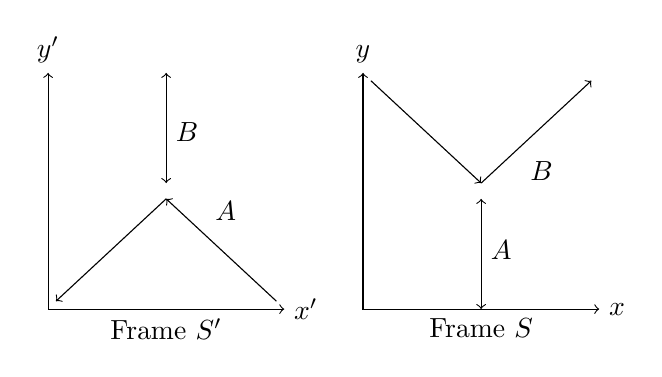
\begin{tikzpicture}
            %\draw[lightgray] (0, 0) grid (7, 3);
            \draw[<->] (3, 0) -- (0, 0) -- (0, 3);
            \draw[<->] (4, 3) -- (4, 0) -- (7, 0);
            \draw[<-] (0.1, 0.1) -- (1.5, 1.4);
            \draw[<-] (1.5, 1.4) -- (2.9, 0.1);
            \draw[<->] (1.5, 1.6) -- (1.5, 3);
            \begin{scope}[xshift=4cm, yscale=-1, yshift=-3cm]
                \draw[->] (0.1, 0.1) -- (1.5, 1.4);
                \draw[->] (1.5, 1.4) -- (2.9, 0.1);
                \draw[<->] (1.5, 1.6) -- (1.5, 3);
            \end{scope}
            \node[below] at (1.5, 0) {Frame \(S'\)};
            \node[below] at (5.5, 0) {Frame \(S\)};
            \node[above right] at (2, 1) {\(A\)};
            \node[below right] at (6, 2) {\(B\)};
            \node[right] at (1.5, 2.25) {\(B\)};
            \node[right] at (5.5, 0.75) {\(A\)};
            \node[right] at (3, 0) {\(x'\)};
            \node[right] at (7, 0) {\(x\)};
            \node[above] at (0, 3) {\(y'\)};
            \node[above] at (4, 3) {\(y\)};
        \end{tikzpicture}
        \caption{Paths of particles \(A\) and \(B\)}
        \label{fig:particle paths}
    \end{figure}
    
    \section{Relativistic Energy}
    \subsection{Particle scattering}
    By symmetry the speed of both particles in the \(y\) direction in their own frames is the same, we will call this speed \(U\).
    \(U\ll c\) so we don't need to consider relativistic effects in the \(y\) direction.
    \[u_B^{(y)'} = u_A^{(y)'} = U\]
    The total change in velocity is two times the velocity as the particle completely changes direction.
    \begin{align*}
        \Delta p_B^{(y)} &= 2k(v)mu_B^{(y)}\\
        &= 2k(v)m\frac{u_B^{(y)'}}{\gamma}\\
        &= 2k(v)m\frac{U}{\gamma}\\
        \Delta p_A^{(y)} &= 2mU\\
        \Delta p_B^{(y)} &= \Delta p_A^{(y)}\\
        2mU &= 2k(v)m\frac{U}{\gamma}\\
        \gamma &= k(v)\\
        \intertext{Hence}
        \vv p &= \gamma m\vv v
    \end{align*}
    A particle moving at high speeds behaves in every way as if its mass has increased by a factor of \(\gamma\).
    Momentum is still conserved once we take this into account.
    
    \subsection{Energy}
    We start in 1D with Newton's second law:
    \[\vv F = \dv{\vv p}{t} = \dv{t}(\gamma m\vv v)\]
    We consider the work done \(dT\) by \(F\) over a small distance \(dx\):
    \[Fdx = dT\]
    \[dT = \dv{(\gamma mv)}{v}dx = m\dv{\gamma v}{t}\]
    \begin{align*}
        \dv{\gamma v}{t}dx &= \gamma\dv{v}{t}dx + v\dv{\gamma}{t}dx\\
        &= \gamma vdv + v^2d\gamma\\
        dT &= \gamma mv dv + mv^2 d\gamma\label{eqn:dT=f(dgamma)}\stepcounter{equation}\tag{\theequation}
    \end{align*}
    \[\gamma = \frac{1}{\sqrt{1- v^2/c^2}}\implies \gamma^2\left(1 - \frac{v^2}{c^2}\right) = 1\implies\gamma^2c^2 = \gamma^2v^2 + c^2\]
    \begin{align*}
    \dv{\gamma}(\gamma^2c^2) &= \dv{\gamma}(\gamma^2v^2 + c^2)\\
    2c^2\gamma &= \gamma^2\dv{v^2}{\gamma} + 2v^2\gamma\\
    2c^2\gamma &= 2v\gamma^2\dv{v}{\gamma} + 2v^2\gamma
    \end{align*}
    \[c^2 = \gamma v\dv{v}{\gamma} + v^2\]
    \[c^2d\gamma = \gamma vdv + d\gamma v^2\]
    From equation \ref{eqn:dT=f(dgamma)}
    \[dT = \gamma mvddv + mv^2d\gamma = m(\gamma vdv + v^2d\gamma) = m(c^2 d\gamma) = mc^2 d\gamma\]
    \[\int dT = mc^2\int d\gamma\]
    \[T = mc^2\gamma + A\]
    for some constant of integration \(A\).
    To find \(A\) consider the case \(T = 0\).
    This means that \(v = 0\) and therefore \(\gamma = 1\).
    \[0 = mc^2 + A\implies A = -mc^2\]
    \[T = mc^2\gamma - mc^2 = (\gamma - 1)mc^2\]
    We can use the binomial expansion
    \[\gamma = 1 + \frac{v^2}{2c^2}\]
    at low speeds
    \[T = (1 + \frac{v^2}{2c^2} - 1)mc^2 = \frac{v^2}{2c^2}mc^2 = \frac{1}{2}mv^2\]
    so this agrees with classical predictions for small \(v\).
    The total energy is given by the rest energy \(mc^2\) and the kinetic energy \(T\) (potential energies are ignored at relativistic speeds as the particles have to be essentially unbounded to be going fast enough)
    \[E = mc^2 + (\gamma - 1)mc^2 = \gamma mc^2\]
    
    \subsection{Energy-Momentum Relation}
    \begin{align*}
        E^2 - p^2c^2 &= \gamma^2m^2c^4 - p^2c^2\\
        &= \gamma^2m^2c^4 - (\gamma mv)^2c^2\\
        &= \gamma^2 m^2c^4\left(1 - \frac{v^2}{c^2}\right)\\
        &= \gamma^2m^2c^4\gamma^{-2}\\
        &= m^2c^4\\
        E^2 &= m^2c^4 + p^2c^2\stepcounter{equation}\tag{\theequation}\label{eqn:energy-momentum relation}
    \end{align*}
    Equation \ref{eqn:energy-momentum relation} is the energy-momentum relation. 
    In it \(m^2c^4\) is the component due to the rest mass, this is constant in all inertial frames, and \(p^2c^2\) is the energy of a photon and is frame dependent.
    This relation holds in all inertial frames so we can use it to equate kinetic energy and momentum and solve for \(v\).
    
    \part{Quantum Mechanics}
    \section{Early Quantum Mechanics}
    \subsection{Black Body Radiation}
    A black body is a body that absorbs all incident thermal radiation.
    It appears black unless it is hot enough to be self luminescent.
    
    A cavity radiator is a good approximation of a black body, it is a hollow body with a small opening, radiation enters the opening and bounces around inside before being `emitted' and leaving through the opening.

    \begin{figure}[ht]
        \centering
        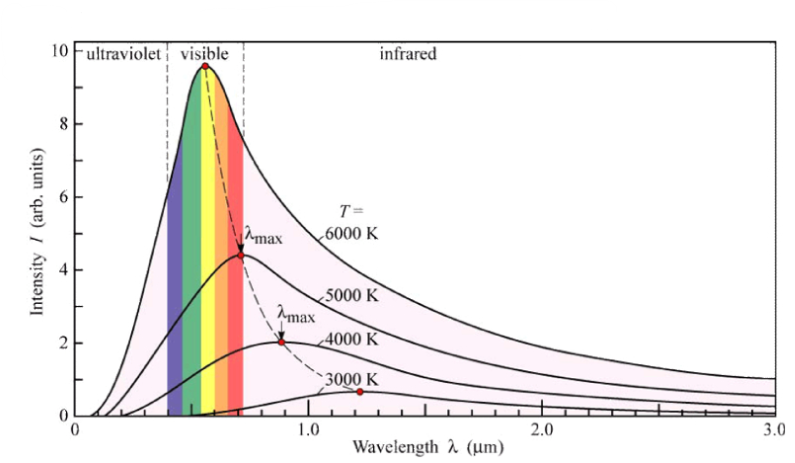
\includegraphics{black_body_radiation.png}
        \caption{Black body radiation wavelength vs intensity for various temperatures}
        \label{fig:black body wavelength vs frequency}
    \end{figure}
    Figure \ref{fig:black body wavelength vs frequency} shows the relative intensity of different wavelengths emitted from a black body depending on the temperature.
    The classical prediction for intensity as a function of wavelength \(u(\lambda)\) is given by the Rayleigh-Jeans law:
    \[u(\lambda) = \frac{8\pi kT}{\lambda^4}\]
    For low values of \(\lambda\) this value tends to infinity but this doesn't match the measured values.
    This is known as the UV catastrophe.
    Planck postulated that electromagnetic radiation has quantised energies.
    This gives rise to the following formulas
    \[\Delta E = hf\]
    \[E_n = nhf\text{ where }n=1,2,3,\dotsc\]
    Combining this gives a different function \(u(\lambda)\) for the intensity:
    \[u(\lambda)=\frac{8\pi hc}{\lambda^5}\frac{1}{e^{hc/\lambda kT} - 1}\]
    This agrees with classical predictions at longer wavelengths and experimental results at shorter wavelengths.
    This is an example of the correspondence principal which states that quantum predictions should agree with classical predictions in the regions where classical predictions agree with experiments.
    
    \subsection{Photoelectric Effect}
    The photoelectric effect occurs when radiation on a metal causes it to emit photoelectrons.
    These electrons have maximum kinetic energy given by
    \[KE_\text{max} = eV_\text{stop} = hf - \varphi\]
    Figure \ref{fig:photoelectric effect graphs} shows two graphs, one shows photocurrent vs applied voltage at two intensities and importantly that both have the same stopping voltage \(V_\text{stop}\). The other shows frequency \(f\) against stopping voltage \(V_\text{stop}\).
    The slope of the line is \(h/e\) and the \(y\) intercept is \(\phi/e\), we can see this by dividing the maximum kinetic energy equation by \(e\) to get
    \[V_\text{stop} = \frac{h}{e}f - \frac{\phi}{e}\]

    \begin{figure}[ht]
        \centering
        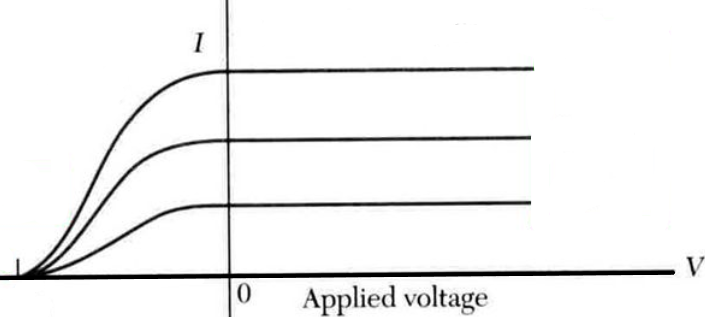
\includegraphics[scale=0.5]{voltage_current_photoelectric_effect.png}
        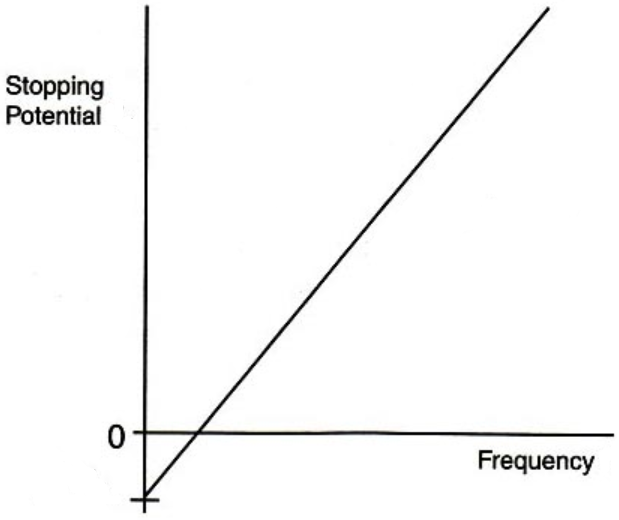
\includegraphics[scale=0.4]{frequency_vs_stopping_potential.png}
        \caption{Graphs of voltage vs current due to the photoelectric effect and frequency vs stopping potential}
        \label{fig:photoelectric effect graphs}
    \end{figure}
    
    Black body radiation and the photoelectric effect are evidence for the particle like nature of light
    
    \subsection{Compton Effect}
    A beam of x-rays is scattered from a graphite target.
    The intensity at different angles is measured.
    We find that there are two peaks in the intensity.
    One peak is at the incident wavelength \(\lambda\).
    The second peak is at a longer wavelength \(\lambda'\) known as the Compton shifted wavelength.
    \[\Delta\lambda = \lambda' - \lambda\]
    \begin{equation}\label{eqn:compton effect}
        \Delta\lambda = \frac{h}{mc}(1 - \cos\vartheta) = \lambda_c(1 - \cos\vartheta)
    \end{equation}
    If we treat the incident radiation as particles hitting an electron we can derive this result from relativistic conservation of energy and momentum.
    Before the collision we choose a rest frame that has the electron stationary.
    The photon has momentum \(p_p = h/\lambda\) and energy \(E_p = p_pc\).
    The electron has momentum \(p_e = 0\) and energy \(E_e = m_ec^2\).
    After the collision the photon travels at an angle of \(\vartheta\) to the axis it was travelling along before the collision.
    The photon has momentum \(p_p' = h/\lambda'\) and energy \(E_p' = p_p'c\).
    The electron has momentum \(p_e'\) and energy \(E_e' = \sqrt{m_e^2c^4 + p_e'^2c^2}\).
    By conservation of linear momentum \(\vv p_e' = \vv p_p + \vv p_e\).
    By conservation of energy \(E_p + E_e = E_p' + E_e'\).
    The energy of the photon is \(E = mc^2 = hf = hc/\lambda\implies \lambda = h/mc\).
    These results can be combined to derive equation \ref{eqn:compton effect}.
    
    De Broglie proposed that this particle-wave like nature applied to matter too.
    He hypothesised that a particle would act as if it had wavelength \(\lambda\) given by
    \[\lambda = \frac{h}{p}\]
    this is known as the De Broglie wavelength of the particle.
    
    \section{The Bohr Model}
    The Bohr model comes from four postulates:
    \begin{enumerate}
        \item An electron in an atom moves in circular orbits under the influence of (classical) Coulomb attraction between the electron and the nucleus.
        \item Electrons only move in orbits for which the angular momentum \(L\) is restricted to integer multiples of \(\hbar\).
        \[L = n\hbar\quad n\in\bb N\]
        \item An electron in an allowed orbit does not radiate energy even though it is accelerating.
        \item Radiation is only emitted if an electron changes from one allowed orbit to another. 
        The frequency of this radiation depends on the energies of the initial and final energy levels, \(E_i\) and \(E_f\) respectively
        \begin{equation}\label{eqn:f=(E1-E2)/h}
            f = \frac{E_i - E_f}{h}
        \end{equation}
    \end{enumerate}
    
    \subsection{Quantisation of Angular Momentum}
    Electrons can be though of as travelling in circular standing waves.
    Which have the relation \(n\lambda = 2\pi r\) for \(n\in \bb N\)
    The angular momentum \(\vv L\) of an electron is
    \[\vv L = \vv r \times \vv p\]
    where \(\vv r\) is its displacement from the centre of the atom and \(\vv p\) is its momentum.
    The electron is travelling slowly enough that we don't need to consider relativistic effects so its momentum is \(\vv p = m\vv v\).
    Its velocity \(\vv v\) is at right angles to \(\vv r\).
    \[L =  |\vv r\times\vv p| = rp\sin\frac{\pi}{2} = rp\]
    The De Broglie wavelength gives us
    \[p = \frac{h}{\lambda}\]
    We can rearrange the standing wave equation to get
    \[r = \frac{n\lambda}{2\pi}\]
    which allows us to eliminate \(r\) from the angular momentum
    \[L = rp = \frac{n\lambda}{2\pi}\frac{h}{\lambda} = n\hbar\quad \text{where }n\in\bb N\]
    This shows us that angular momentum is quantised for an electron in an atomic orbit.
    
    \subsection{Orbit Radius}
    We can balance the centripetal and electrostatic forces
    \begin{equation}\label{eqn:centripetal=electrostatic}
        \frac{mv^2}{r} = \frac{1}{4\pi\varepsilon_0}\frac{e^2}{r^2}
    \end{equation}
    From before we have
    \begin{equation}\label{eqn:angular momentum}
        L = rp = rmv = n\hbar\implies v = \frac{n\hbar}{rm}
    \end{equation}
    we substitute this into equation \ref{eqn:centripetal=electrostatic} to get
    \begin{equation}\label{eqn:orbit radius}
        r = \frac{4\pi\varepsilon_0\hbar^2}{me^2}n^2\quad\text{where }n\in\bb N
    \end{equation}
    The smallest possible value of this is at \(n = 1\).
    We get \(r = \SI{0.0529}{nm}\), this is known as the Bohr radius.
    If instead we rearrange equation \ref{eqn:angular momentum} to find \(r\) we get
    \[r = \frac{n\hbar}{vm}\]
    Substituting this into equation \ref{eqn:centripetal=electrostatic} we get
    \[v = \frac{e^2}{4\pi\varepsilon_0\hbar n}\]
    The largest value that this can take is at \(n = 1\) where we get \(v\approx \SI{2e6}{m.s^{-1}}\ll c\) so we don't need to consider relativistic effects.
    
    \subsection{Quantisation of Energy}
    From equation \ref{eqn:centripetal=electrostatic} we get
    \[KE = \frac{1}{2}mv^2 = \frac{e^2}{4\pi\varepsilon_02r}\]
    We can calculate the potential energy as the negative integral of electrostatic force.
    The limits are \(r\) and \(\infty\) as this is the limit of where the electron can be
    \[PE = -\int_r^\infty\frac{e^2}{4\pi\varepsilon_0 r^2}\,dr = -\frac{e^2}{4\pi\varepsilon_0 r}\]
    This means the total energy \(E\) is
    \[E = KE + PE = -\frac{e^2}{4\pi\varepsilon_02r}\]
    Substituting the value for \(r\) from equation \ref{eqn:orbit radius} we get
    \[E = -\frac{me^4}{(4\pi\varepsilon_0)^22\hbar^2n^2}\quad\text{where }n\in\bb N\]
    Substituting this into equation \ref{eqn:f=(E1-E2)/h} we get
    \[\frac{1}{\lambda} = R_H\left(\frac{1}{n_f^2} - \frac{1}{n_i^2}\right)\]
    where \(n_i\) and \(n_f\)are the initial and final values of \(n\) respectively and \(R_H\) is the Rydberg constant
    \[R_H = \left(\frac{1}{4\pi\varepsilon_0}\right)^2\frac{me^4}{4\pi\hbar^3c} = \frac{me^4}{8\varepsilon_0^2h^3c}\]
    
    \subsection{Limitations of the Bohr Model}
    The Bohr model has several draw backs:
    \begin{itemize}
        \item It only works for hydrogen like atoms/ions, that is atoms that have been ionised to such that they have one remaining electron.
        For non hydrogen like atoms we need another model, like the Scr\"odinger equation.
        \item In this model we assume we know the location of the electrons and their momentum, this violates uncertainty.
        \item This model doesn't explain why some allowed transitions are more likely than others just whether or not a transition is allowed.
        \item The Bohr model lacks coherence, it mixes classical and non-classical concepts and just ignores some explicitly in the postulates.
    \end{itemize}

    \section{The Wave Function}
    \subsection{Double Slit}
    \[m\lambda = d\sin\vartheta\]
    where \(m\in\bb Z\), \(d\) is the slit separation, \(\vartheta\) is the angle of diffraction and \(\lambda\) is the wavelength.
    Even if one electron at a time is sent through the slits we still get interference.
    If we try to observe the electron going through a slit the electrons that we observe only pass through one slit and no interference occurs.
    The electrons that we fail to observe will still have an interference pattern.
    
    \subsection{Wave-Particle Model}
    For radiation:
    
    The wave model has intensity \(I\) proportional to the square of the electric field \(E\)
    \[I\propto E^2\]
    The particle model has intensity proportional to the photon density \(N\)
    \[I\propto N\]
    Combining these we get
    \[I\propto E^2\propto N\]
    We interpret \(E^2\) as a probability measure of photon density.
    
    For matter:
    
    The analogous function for matter is the wave function \(\psi(x, t)\).
    The probability of finding a particle in a small region of space around \(x\) at time \(t\) is given by the probability density function (pdf) \(P\):
    \[P(x, t) = |\psi(x, t)|^2 = \psi(x, t)\psi^*(x, t)\]
    where \(^*\) denotes the complex conjugate.
    The wave function describes where the particle \emph{may} be found, not where it \emph{will} be found.
    There is no concept of a trajectory in this model.
    \subsection{Wave Functions}
    To combine wave functions \(\psi_1\) and \(\psi_2\) we simply add them to get
    \[\psi = \psi_1 + \psi_2\]
    To find the pdf of the resulting wave function \(\psi\) we square \(\psi\):
    \begin{align*}
        P &= |\psi|^2\\
        &= |\psi_1 + \psi_2|^2\\
        &= (\psi_1 + \psi_2)(\psi_1 + \psi_2)^*\\
        &= (\psi_1 + \psi_2)(\psi_1^* + \psi_2^*)\\
        &= \psi_1\psi_1^* + \psi_2\psi_2^* + \psi_1\psi_2^* + \psi_1^*\psi_2\\
        &= |\psi_1|^2 + |\psi_2|^2 + \psi_1\psi_2^* + \psi_1^*\psi_2
    \end{align*}
    
    \subsection{Waves Recap}
    A wave travelling in the \(+x\) direction is given by
    \[y(x, y) = A\sin(kx - \omega t)\]
    where \(A\) is the amplitude, \(k = 2\pi/\lambda\) is the wavenumber and \(\omega = 2\pi f\) is the angular frequency.
    If the sign in front of the \(\omega t\) term was \(+\) instead then this would be a wave travelling in the \(-x\) direction.
    Any function \(F\) of the form \(y(x, t) = F(kx - \omega t)\) represents a travelling wave.
    Euler's identity is \(e^{ix} = \cos x + i\sin x\) which gives us
    \[e^{i(kx - \omega t)} = \cos(kx - \omega t) + i\sin(kx - \omega t)\]
    this represents a wave travelling in the \(+x\) direction.
    
    The wave function of a free particle with energy \(E\) and momentum \(p\), travelling in the \(+x\) direction is
    \[\psi(x, t) = Ae^{i(kx-\omega t)} = Ae^{i(px-Et)/\hbar}\]
    since \(p = h/\lambda = \hbar k\) and \(E = hf = \hbar\omega\).
    
    \subsection{Heisenberg's Uncertainty Principle}
    Heisenberg's uncertainty principle (HUP) relates to the fundamental inability to know certain values to arbitrary accuracy at the same time.
    Its two most common forms are:
    \[\Delta p_x\Delta x\ge \frac{\hbar}{2}\]
    \[\Delta E\Delta t\ge \frac{\hbar}{2}\]
    where \(\Delta a\) denotes uncertainty in \(a\)
    For a free particle \(k\) is known and hence \(p\) is known so \(\Delta p = 0\).
    The only way that this can be true is if \(\Delta x = \infty\).
    We can try to find \(x\) from the wave function:
    \begin{align*}
        |\psi(x, t)|^2 &= |Ae^{i(kx-\omega t)}|^2\\
        &= Ae^{i(kx-\omega t)}A^*e^{-i(kx-\omega t)}\\
        &= AA^*\\
        &= |A|^2
    \end{align*}
    This is constant for all \(x\) so the location of the particle is undefined, it is equally likely to be anywhere.
    
    \section{Schr\"odinger's Theory}
    \subsection{Uncertainty Principle Examples}
    \example
    A bullet mass \SI{50}{g} and an electron mass \SI{9.1e-31}{kg} are travelling at a measured speed of \(\SI{300}{m.s^{-1}}\) with uncertainty of \SI{0.01}{\%}.
    What is the accuracy in measuring the position?
    \[\Delta p\Delta x \ge \frac{\hbar}{2}\]
    \[\Delta p = m\Delta v\]
    \[\Delta x \ge \frac{\hbar}{2m\Delta v}\]
    For the bullet \(m = \SI{0.05}{kg}\), \(\Delta v = \SI{0.07}{m.s^{-1}}\):
    \[\Delta x \ge \SI{3e-33}{m}\]
    For the electron \(m = \SI{9.1e-31}{kg}\), \(\Delta v = \SI{0.08}{m.s^{-1}}\):
    \[\Delta x \ge \SI{0.2}{cm}\]
    As expected this value is much larger for the electron and basically negligible on a macroscopic scale.
    
    \example
    The initial positions of a \SI{1}{kg} object and an electron are known to within one nuclear radius \((\SI{e-14}{m})\) and their initial velocities are known to the accuracy allowed by the uncertainty principle.
    Assume no force acts on the objects.
    Find their position uncertainties one year later.
    
    At \(t = 0\)
    \[\Delta p\Delta x_0 \ge \frac{\hbar}{2}\]
    \[\Delta v \ge \frac{\hbar}{2m\Delta x_0}\]
    At time \(t\):
    \[\Delta x_t = t\Delta v \ge\frac{\hbar t}{2m\Delta x_0}\]
    \(\Delta x_0 = \SI{e-14}{m}\), \(t = \SI{3.2e6}{s}\), for the object \(m = \SI{1}{kg}\):
    \[\Delta x_t \ge \SI{2e-13}{m}\]
    For the electron \(m = \SI{9.1e-31}{kg}\):
    \[\Delta x_t \ge \SI{2e17}{m}\]
    For comparison the size of the solar system is \(\SI{e12}{m}\)
    
    \subsection{Schr\"odinger Equation}
    For electromagnetic radiation the wave equation is
    \[\pdv[2]{E}{x} = \frac{1}{c^2}\pdv[2]{E}{t}\]
    The analogous function for matter is
    \[\frac{-h^2}{2m}\pdv[2]{\psi}{x} = i\hbar\pdv{\psi}{t}\]
    
    Schr\"odinger's theory of quantum mechanics specifies the Schr\"odinger equation, which controls the wave function, and a connection between the wave function and how the particle acts.
    It agrees with Newton in the macroscopic limit.
    
    \subsection{Classical Wave Equation}
    \[\pdv[2]{y(x, t)}{x} = \frac{1}{v^2}\pdv[2]{y(x, t)}{t}\]
    where \(v = \omega/k\) is the speed of the wave.
    The solutions to this are \(y(x, t) = F(kx-\omega t)\).
    This can be shown by differentiating and showing that the equation holds:
    \[\pdv{F}{x} = kF(kx-\omega t),\qquad \pdv[2]{F}{x} = k^2F(kx - \omega t)\]
    \[\pdv{F}{t} = -\omega F(kx - \omega t),\qquad \pdv[2]{F}{t}=\omega^2F(kx - \omega t)\]
    \[k^2F(kx-\omega t) = \frac{k^2}{\omega^2}\omega^2F(kx-\omega t)\]
    
    \section{Schr\"odinger Equation}
    In order to make a plausibility argument for the Schr\"odinger equation we need to make several assumptions about the wave equation.
    The wave equation must be:
    \begin{itemize} 
        \item Linear in wave function \(\psi(x, t)\) so waves can be added to produce an interference pattern
        \item Consistent with the De Broglie--Einstein relations:
        \[p = \frac{h}{\lambda} = \hbar k\]
        \[E = hf = \hbar \omega\]
        \item Consistent with the equation for total energy:
        \[E = KE + PE = \frac{p^2}{2m} + V(x, t)\]
        \item For the special case of a free particle:
        \begin{itemize}
            \item Have constant linear momentum \(p\) and total energy \(E\)
            \item The solution is assumed to have the form of a sinusoidal travelling wave (hence \(\lambda\) and \(f\) are constant)
        \end{itemize}
    \end{itemize}
    We start with the total energy with constant potential \(V_0\)
    \[E = \frac{p^2}{2m} + V_0\]
    and we substitute \(E=\hbar \omega\) and \(p = \hbar k\) to get
    \begin{equation}\label{eqn:total energy}
        \hbar \omega = \frac{\hbar^2k^2}{2m} + V_0
    \end{equation}
    First we will show that the most basic wave is \emph{not} as solution.
    We can do this by showing that after substitution one side of the Schr\"odinger equation is proportional to \(\psi(x, t)\) and the other isn't.
    \[\psi(x, t) = A\sin(kx - \omega t)\]
    \[\pdv[2]{\psi}{x} = -k^2A\sin(kx - \omega t) = -k^2\psi(x, t)\propto \psi(x, t)\]
    \[\pdv{\psi}{t} = -\omega A\cos(kx-\omega t)\not\propto \psi(x, t)\]
    This is a contradiction so \(\psi(x, t) = A\sin(kx - \omega t)\) is not a solution.
    
    Due to our assumptions it is possible to try linear combinations of \(\sin(kx - \omega t)\) and \(\cos(kx - \omega t)\). 
    We find that one in particular works:
    \[\psi(x, t) = A(\cos(kx - \omega t) + i\sin(kx - \omega t) = Ae^{i(kx - \omega t)}\]
    We can work out \(k\) and \(\omega\) in terms of derivatives of \(\psi(x, t)\) by substituting this in to the Scr\"odinger equation
    \[\pdv[2]{\psi}{x} = i^2k^2Ae^{i(kx - \omega t)} = -k^2Ae^{i(kx - \omega t)} = -k^2\psi\implies k^2 = -\pdv[2]{\psi}{x}\frac{1}{\psi}\]
    \[\pdv{\psi}{t} = -i\omega Ae^{i(kx-\omega t)} = -i\omega\psi \implies \omega = -\pdv{\psi}{t}\frac{1}{i\psi} = \pdv{\psi}{t}\frac{i}{\psi}\]
    We can then substitute these into equation \ref{eqn:total energy} to get
    \[i\hbar\pdv{\psi}{t}\frac{1}{\psi} = -\frac{\hbar^2}{2m}\pdv[2]{\psi}{x}\frac{1}{\psi} + V_0\]
    \[i\hbar\pdv{\psi}{t} = -\frac{\hbar^2}{2m}\pdv[2]{\psi}{x} + V_0\psi\]
    We make the (completely unjustified) assumption that this holds for non-constant potential \(V(x, t)\):
    \[i\hbar\pdv{\psi}{t} = -\frac{\hbar^2}{2m}\pdv[2]{\psi}{x} + V(x, t)\psi(x, t)\]
    This is the time dependent Schr\"odinger equation.
    It is linear in wave function so we can do superposition.
    It is first order in time so the solution only requires one set of boundary conditions, usually at \(t = 0\).
    The presence of \(i\) means that \(\psi:\bb R^2\to \bb C\) so the wave function can't be measured directly as it is complex.
    We can measure its square \(|\psi|^2 = \psi^*\psi\) as this is real.
    There is no concept of trajectory in this equation.
    There is no quantisation (yet).
    This comes when we define \(V\).
    
    \subsection{Observables and Operators}
    Observables are properties which can be measured experimentally.
    For example position, momentum or energy.
    In classical physics observables are represented by variables. For example \(x(t)\), \(\vv p(t)\) or \(E(x, t)\).
    In quantum mechanics observables are represented by linear operators which act on the wave function (actually they are the real eigenvalues of these operators).
    This is a postulate of quantum mechanics.
    
    An operator is commonly denoted by a hat eg \(\hat L\).
    A linear operator \(\hat L\) is a mapping between two vector spaces.
    What this means for our needs is that it acts on a function and returns another function (as functions are members of a vector space).
    The property of being linear is defined as the following holding:
    \begin{itemize}
        \item For functions \(f\) and \(g\) and linear operator \(\hat L\): \(\hat L(f + g) = \hat Lf + \hat Lg\)
        \item For function \(f\), scalar \(c\) and linear operator \(\hat L\): \(\hat L(cf) = c\hat Lf\)
    \end{itemize}
    
    \subsection{Momentum and Position Operators}
    We can derive the momentum operator \(\hat p\) for a free particle from its wave function:
    \[\psi(x, t) = Ae^{i(px - Et)/\hbar}\]
    \[\pdv{\psi}{x} = \frac{ip}{\hbar}Ae^{i(px - Et)/\hbar} = \frac{ip}{\hbar}\psi(x, t)\]
    \[p\psi(x, t) = -i\hbar\pdv{x}\psi(x, t)\]
    There is an association:
    \[p\leftrightarrow -i\hbar\pdv{x}\]
    The momentum operator \(\hat p\) is
    \[\hat p = -i\hbar\pdv{x}\]
    It is clear that \(p\) is an eigenvalue of \(\hat p\) and therefore observable since by definition:
    \[\hat p\psi(x, t) = p\psi(x, t)\]
    The position operator is \(\hat x = x\) since this gives
    \[\hat x\psi(x, t) = x\psi(x, t)\]
    and \(x\) is clearly the eigenvalue of this operator.
    We make the assumption that these operators are the same for all \(\psi(x, t)\) not just for a free particle.
    
    \section{Probability Density Function}
    \subsection{Hamiltonian}
    The kinetic energy is classically given by \(T = p^2/2m\) from this we get that the kinetic energy operator \(\hat T\) is given by
    \[\hat T = \frac{\hat p^2}{2m} = \frac{1}{2m}\left(-i\hbar\pdv{x}\right)\left(-i\hbar\pdv{x}\right) = -\frac{\hbar^2}{2m}\pdv[2]{x}\]
    The total energy operator is called the Hamiltonian and is denoted \(\hat H\). It is given by
    \[\hat H = \hat T + \hat V\]
    where \(\hat V\) is the potential energy operator, \(\hat V = V(x, t)\)
    \[\hat H = -\frac{\hbar^2}{2m}\pdv[2]{x} + V(x, t)\]
    We can compare this with the time dependent Schr\"odinger equation:
    \[\underbrace{\left[-\frac{\hbar^2}{2m}\pdv[2]{x} + V(x, t)\right]}_{\hat H}\psi(x, t) = i\hbar\pdv{t}\psi(x, t)\]
    This allows us to write the time dependent Schr\"odinger equation in the condensed form
    \[\hat H\psi(x, t) = i\hbar \pdv{t}\psi(x, t)\]
    which allows us to see that
    \[\hat H = i\hbar\pdv{t}\]
    All of the operators mentioned so far are linear and Hermitian.
    This means that they have real eigenvalues.
    
    \subsection{Probability Recap}
    \(P(x)\) is the probability density function (pdf) of random variable \(x\).
    The expected value of \(x\) is denoted \(\expected x\).
    For a discrete \(x\) that can take the values \(x_1, x_2, \dotsc, x_n\) the expected value is calculated as
    \[\expected{x} = \sum_{i=1}^nx_iP(x_i)\]
    
    One classical example where probability is used is in radioactive decay.
    The lifetime \(t\) of a particle can be modelled as a random variable where \( t\in [0, \infty]\).
    We define
    \[P(t)dt\]
    as the probability that the lifetime of the particle is in the range \([t, t + dt]\).
    We calculate the expected value of \(t\) as
    \[\expected{t} = \int_0^\infty tP(t)\,dt\]
    since \(t\) is continuous the sum becomes an integral.
    It can be shown that \(P(t) = \lambda e^{-\lambda t}\).
    The factor of \(\lambda\) comes from the restriction that since the particle must decay at some point
    \[\int_0^\infty P(t)\,dt = 1\]
    and \(P(t) = Ae^{-\lambda t}\) so
    \[\int_0^\infty P(t)\,dt = \left[-\frac{1}{\lambda}Ae^{-\lambda t}\right]_0^\infty = \frac{A}{\lambda} = 1 \implies A = \lambda\]
    Hence the expected value of \(t\) can be calculated as
    \[\expected{t} = \int_0^\infty tP(t)\,dt = \frac{1}{\lambda} = \tau\]
    where \(\tau\) is defined as the expected lifetime of the particle.
    
    \subsection{Quantum Probability}
    For a particle with wave function \(\psi(x, t)\) the probability density function is defined as
    \[P(x, t) = |\psi(x, t)|^2 = \psi^*(x, t)\psi(s, t)\]
    where \(^*\) denotes the complex conjugate.
    The probability that a particle is in a range \([x, x + dx]\) is given by
    \[P(x, t)dx\]
    The probability that a particle is in a range \([a, b]\) is given by
    \[\int_a^bP(x, t)\,dx\]
    It is worth noting that
    \[\int_a^a P(x, t)\,dx = 0\A a\]
    so the probability of any particular value of \(x\) is 0.
    Since the particle is somewhere in space
    \[\int_{-\infty}^\infty P(x, t)\,dx = 1\]
    Setting this condition is called normalisation.
    This is ok as if \(\psi\) is a wave function then so is \(c\psi\) where \(c\in \bb R\) this allows us to scale \(\psi\) such that it is normalised.
    To be normalised a wave function must be square integrable, that is
    \[\int_{-\infty}^\infty |\psi(x, t)|^2\,dx\]
    must exist and be finite.
    For most cases this means that \(\psi(x, t)\to 0\) as \(x\to\pm\infty\).
    
    The expected position is given by
    \[\expected{x} = \int_{-\infty}^\infty xP(x, t)\,dx = \int_{-\infty}^\infty \psi^*(x, t)x\psi(x, t)\,dx\]
    Likewise for momentum we can find \(\expected{p}\) using \(\hat p\):
    \[\expected{p} = \int_{-\infty}^\infty \psi^*(x, t)\hat p\psi(x, t)\,dx\]
    Note that this means that the order of the terms in the integrand is important as \(\psi^*\hat p\psi\ne \hat p\psi^*\psi\).
    Technically \(\psi\hat p\psi^*\) is also valid but by convention we put \(\psi^*\) first.
    We can generalise this to any observable \(A\) with operator \(\hat A\):
    \[\expected{A} = \int_{-\infty}^\infty \psi^*(x, t)\hat A\psi(x, t)\,dx\]
    
    If we have an infinite number of identical systems the expected value is the average value of an observable measured once in each system.
    It is \emph{not} the expected value after multiple measurements of one system as this will disturb the system, or the expected value of one measurement as this is best described by a distribution rather than a single value.
    
    We can also find quantitative information about uncertainty.
    The uncertainty in \(A\) is \(\Delta A\).
    It is given by
    \[\Delta A^2 = \expected{(A - \expected{A})^2} \implies \Delta A = \sqrt{\expected{(A - \expected{A})^2}}\]
    that is the average distance from the expected value.
    We can simplify this statement using a few properties of the expected value:
    \begin{itemize}
        \item \(\expected{a + b} = \expected{a} + \expected{b}\) for two unrelated values \(a\) and \(b\)
        \item \(\expected{k} = k\) for constant \(k\). Note that the expected value of a variable is itself a constant so \(\expected{\expected{a}} = \expected{a}\).
        \item \(\expected{ka} = k\expected{a}\) for constant \(k\).
    \end{itemize}
    \begin{align*}
        \expected{(A - \expected{A})^2} &= \expected{A^2 - 2A\expected{A} + \expected{A}^2}\\
        &= \expected{A^2} - \expected{2A\expected{A}} + \expected{A}^2\\
        &= \expected{A^2} - 2\expected{A}\expected{A} + \expected{A}^2\\
        &= \expected{A^2} - \expected{A}^2
    \end{align*}
    \[\Delta A = \sqrt{\expected{A^2} - \expected{A}^2}\]
    
    \subsection{Probability With Dirac Notation}
    The inner product of two functions with domains \([a, b]\) is defined as
    \[\braket{f}{g} = \int_a^bf^*(x)g(x)\,dx\]
    The wave function is a function with domain \([-\infty, \infty]\) so we can restate the normalisation condition as
    \[\braket{\psi}{\psi} = 1\]
    We can also use Dirac notation to define the expected value by defining
    \[\braopket{f}{\hat A}{g} = \braket{f}{\hat Ag} = \int_a^bf^*(x)\hat Ag(x)\,dx\]
    for functions \(f\) and \(g\) with domains \([a, b]\) and operator \(\hat A\).
    This means that the expected value of \(A\) is given by
    \[\expected{A} = \braopket{\psi}{\hat A}{\psi}\]
    
    \section{Time Independent Schr\"odinger Equation}
    The time dependant Schr\"odinger equation for wave function \(\Psi(x, t)\) is
    \begin{equation}\label{eqn:TDSE}
        -\frac{\hbar^2}{2m}\pdv[2]{\Psi(x, t)}{x} + V(x, t)\Psi(x, t) = i\hbar\pdv{\Psi(x, t)}{t}
    \end{equation}
    We assume the existence of solutions of the form
    \[\Psi(x, t) = \psi(x)\varphi(t)\]
    Substituting this into equation \ref{eqn:TDSE} we get
    \[-\frac{\hbar^2}{2m} \varphi(t) \dv[2]{\psi(x)}{x} + V(x, t) \psi(x) \varphi(t) = i\hbar \psi(x) \dv{\varphi(t)}{t}\]
    We assume that \(V = V(x)\) (ie the potential is constant with time) and divide through by \(\psi(x)\varphi(t)\) to get
    \[\frac{1}{\psi(x)}\left[\frac{-\hbar^2}{2m} \dv[2]{\psi(x)}{x} + V(x)\psi(x)\right] = \frac{i\hbar}{\varphi(t)}\dv{\varphi(t)}{t}\]
    The left hand side depends only on \(x\) and the right hand side depends only on \(t\).
    The only way that this can be true is if both sides are equal to some constant \(C\)
    \begin{equation}\label{eqn:space part of separated TDSE}
        \frac{1}{\psi(x)}\left[-\frac{\hbar^2}{2m}\dv[2]{\psi(x)}{x} + V(x)\psi(x)\right] = C
    \end{equation}
    \begin{equation}\label{eqn:time part of separated TDSE}
        \frac{i\hbar}{\varphi(t)}\dv{\varphi(t)}{t} = C
    \end{equation}
    We now have two ODE in \(x\) and \(t\).
    We can rearrange equation \ref{eqn:time part of separated TDSE} to get
    \[\dv{\varphi(t)}{t} = -\frac{iC}{\hbar}\varphi(t)\]
    Which has solutions of the form
    \[\varphi(t) = e^{-iCt/\hbar}\]
    This is a function oscillating in time with frequency \(\omega = C/\hbar\).
    We know from the Planck-Einstein relation that \(\omega = E/\hbar\) therefore \(C = E\).
    This gives
    \[\varphi(t) = e^{-iEt/\hbar}\]
    Substituting \(C = E\)  into equation \ref{eqn:space part of separated TDSE} we get
    \[-\frac{\hbar^2}{2m}\dv[2]{\psi(x)}{x} + V(x)\psi(x) = E\psi(x)\]
    This is the time independent Schr\"odinger equation.
    The original wave function is given by
    \[\Psi(x, t) = \psi(x)e^{-iEt/\hbar}\]
    The time independent Schr\"odinger equation is linear in \(\psi(x)\).
    It also doesn't contain \(i\) so \(\psi(x)\) can be a real function.
    The solutions may only exist for certain values of \(E\) so we get quantisation.
    
    \subsection{Eigenvalue Equations}
    In general a linear operator \(\hat A\) operating on a function \(f\) returns another function
    \[\hat Af(x) = g(x)\]
    Sometimes it returns a scalar multiple of the original function
    \[\hat Af(x) = af(x)\]
    this is called an eigenvalue equation.
    \(f\) is known as an eigenfunction of \(\hat A\) and \(a\) is its corresponding eigenvalue.
    
    We can write the time dependent Schr\"odinger equation as an eigenvalue equation for the Hamiltonian
    \[\left(-\frac{\hbar^2}{2m}\dv[2]{x} + V(x)\right)\psi(x) = E\psi(x)\]
    \[\hat H \psi(x) = E\psi(x)\]
    here \(\psi\) is an eigenfunction and \(E\) is the eigenvalue.
    The system is said to be in an energy eigenstate - it has a definite value of \(E\).
    
    \subsection{Stationary States}
    The probability density function of the solutions to the time independent Schr\"odinger equation is
    \begin{align*}
        P(x, t) &= \Psi^*(x, t)\Psi(x, t)\\
        &= \psi^*(x)e^{iEt/\hbar}\psi(x)e^{-iEt/\hbar}\\
        &= \psi^*(x)\psi(x)\\
        &= |\psi(x)|^2
    \end{align*}
    So wave functions of the form \(\Psi(x, t) = \psi(x)e^{-iEt/\hbar}\) are called stationary states as \(P(x, t)\) doesn't vary with time.
    
    \section{Commutators}
    \subsection{General Solution to TISE}
    There is often more than one eigenfunction of \(\hat H\).
    The solutions to the time independent Schr\"odinger equation at energies \(E_n\) satisfy
    \[\hat H\psi_n(x) = E_n\psi_n(x)\]
    This gives solutions to the time dependent Schr\"odinger equation:
    \[\Psi_n(x, t) = \psi_n(x)e^{-iE_nt/\hbar}\]
    The general solution is then a linear combination of these
    \[\Psi(x, t) = \sum_{n = 1}^\infty c_n \Psi_n(x, t) = \sum_{n = 1}^\infty c_n \psi_n(x)e^{-iE_nt/\hbar}\]
    where the constant \(c_n\) are normalisation coefficients.
    
    \subsection{Commutativity}
    The commutator of two operators \(\hat A\) and \(\hat B\) is defined as
    \[[\hat A, \hat B] = \hat A\hat B - \hat B\hat A\]
    If \([\hat A, \hat B] = 0\) then \(\hat A\) and \(\hat B\) are said to commute.
    
    Suppose a quantum mechanical particle is in a state \(\psi(x)\) which has a definite value \(a\) of an observable \(A\) with operator \(\hat A\).
    Then \(\psi(x)\) is an eigenfunction of \(\hat A\) with eigenvalue \(a\):
    \[\hat A\psi(x) = a\psi(x)\]
    If we can simultaneously measure a definite value \(b\) of an observable \(B\) with operator \(\hat B\) then this must also give an eigenvalue equation
    \[\hat B\psi(x) = b\psi(x)\]
    It is only possible to make these two measurements simultaneously if \(\hat A\) and \(\hat B\) commute, that is \([\hat A, \hat B] = 0\).
    If they don't commute then there is a related uncertainty principle.
    
    \example
    We do not expect \(\hat x\) and \(\hat p\) to commute as there is an uncertainty principle connecting them.
    We can show they do not by applying the commutator \([\hat x, \hat p]\) to a dummy function \(\psi\):
    \begin{align*}
        [\hat x, \hat p]\psi &= \left[x\left(-i\hbar\pdv{x}\right) - \left(-i\hbar\pdv{x}\right)x\right]\psi\\
        &= -i\hbar x\pdv{x}\psi + i\hbar \pdv{x}[x\psi]\\
        &= -i\hbar x\pdv{\psi}{x} + i\hbar \pdv{x}{x}\psi + i\hbar \pdv{\psi}{x}\\
        &= i\hbar\psi
    \end{align*}
    Hence \([\hat x, \hat p] = i\hbar \ne 0\) so \(\hat x\)  and \(\hat p\) don't commute and position and momentum can't accurately be measured at the same time.
    
    \section{Solutions to the Schr\"odinger Equation}
    
    There are many solutions that are mathematically feasible for the Schr\"odinger equation.
    Many of these solutions must be disregarded as they don't make physical sense.
    Observables must be physically reasonable.
    This imposes the additional restrictions that the solutions must be ``well behaved".
    That is that \(\psi(x)\) and \(\inlinedv{\psi(x)}{x}\) must be:
    \begin{itemize}
        \item Finite
        \item Single Valued
        \item Continuous
    \end{itemize}
    The reasons for these restrictions is
    \begin{itemize}
        \item \(\psi(x)\) and \(\inlinedv{\psi(x)}{x}\) must be finite and single valued so that the wave function \(\Psi(x, t)\) and its space derivative \(\inlinepdv{\Psi(x, t)}{x}\) are finite and single valued.
        \textit{(\(\psi(x)\) may be infinite at a point as long as the integral of \(\psi^*(x)\psi(x)\) is finite over all regions containing that point)}.
        Which in turn is needed so that the expected values of observables calculated are reasonable.
        \item Continuity of \(\psi(x)\) is needed so that \(\inlinedv{\psi(x)}{x}\) is finite.
        \item Continuity of \(\inlinedv{\psi(x)}{x}\) is needed so that \(\inlinedv[2]{\psi(x)}{x}\) is finite which is needed for solutions involving finite \(\psi(x)\), \(V(x)\) and \(E\).
    \end{itemize}
    Depending on boundary conditions there may or may not be a solution for particular values of \(E\) so we get quantisation of energy.
    
    \subsection{Free Particle}
    For a free particle \(V(x) = 0\).
    We have seen that the valid solutions are
    \[\psi_1(x) = e^{ikx}, \qquad \psi_2(x) = e^{-ikx} \qquad \text{where } k = \frac{\sqrt{2mE}}{\hbar}\]
    \(\psi_1\) gives the solution for a particle travelling in the \(+x\) direction whereas \(\psi_2\) gives the solution for a particle travelling in the \(-x\) direction.
    This gives a general solution of any linear combination of these
    \[\psi(x) = Ae^{ikx} + Be^{-ikx}\]
    This gives solutions to the time dependent Schr\"odinger equation of
    \begin{equation}\label{eqn:free particle general solution}
        \Psi(x, t) = Ae^{i(kx - \omega t)} + Be^{i(-kx - \omega t)}
    \end{equation}
    where \(\omega = E/\hbar\).
    If we know the direction of the particle we can set \(A\) or \(B\) to 0 to get rid of the term travelling in the wrong direction.
    If for example we know the particle is travelling in the \(+x\) direction then \(B = 0\) and \(|\Psi(x, t)|^2 = |A|^2\).
    This is not normalisable since (for a particle travelling in the \(+x\) direction)
    \[\int_{-\infty}^\infty P(x, t)\,dx = |A|^2\int_{-\infty}^\infty dx = \infty\]
    The particle is equally likely to be anywhere since \(P(x, t)\) is constant.
    This means we can measure momentum exactly and if we do we get \(p = \sqrt{2mE}\) for a particle travelling in the \(+x\) direction and \(p = -\sqrt{2mE}\) for a particle travelling in the \(-x\) direction.
    
    \subsection{Constant Potential}
    For a constant potential \(V(x) = V_0\) where \(V_0 < E\).
    The time independent Schr\"odinger equation is then
    \[-\frac{\hbar^2}{2m}\dv[2]{\psi(x)}{x} = (E - V_0)\psi(x)\]
    This has the same general solutions as a free particle given in equation \ref{eqn:free particle general solution} but now
    \[k = \frac{\sqrt{2m(E - V_0)}}{\hbar}\]
    It is clear that the free particle is just a special case of this with \(V_0 = 0\).
    Since potentials are measured relative by redefining ``zero energy" we can simplify this to the free particle case.
    
    \subsection{High Energy Step}
    \[
        V(x) =
        \begin{cases}
            0 & x < 0\\
            V_0 & x\ge 0
        \end{cases}
    \]
    where \(V_0 > E\). Classically we would expect a particle travelling in the \(+x\) direction to be reflected upon reaching the boundary.
    This is not what we see in quantum mechanics.
    To solve this and many other potentials given by a piecewise function there is a consistent method:
    \begin{enumerate}
        \item Solve the time independent Schr\"odinger equation in each region
        \item Ensure solutions are physically reasonable
        \item Join the solutions using the boundary conditions that \(\psi(x)\) and \(\inlinedv{\psi(x)}{x}\) are smooth at the boundary
    \end{enumerate}
    Region 1:
    \[-\frac{\hbar^2}{2m}\dv[2]{\psi_1}{x} = E\psi_1(x)\]
    This is a free particle hence
    \[\psi_1(x) = Ae^{ik_1x} + Be^{-ik_1x}\qquad\text{where }k_1\frac{\sqrt{2mE}}{\hbar}\]
    This is physically reasonable, the first term is the wave travelling in the \(+x\) direction and the second term is the reflected part of the wave.
    
    Region 2:
    
    Since in the classical limit we expect that the particle would not be in the region \(x \ge 0\) (henceforth the classically forbidden region) the wave function in this region must decay to 0.
    We propose
    \[\psi_2(x) = Ce^{k_2x} + De^{-k_2x}\]
    as a solution.
    It is simple to show that this is a solution to the time independent Schr\"odinger equation.
    We must ask if this is physically reasonable.
    The \(De^{-ke_2x}\) term decays to 0 as \(x\to \infty\) but the \(Ce^{k_2x}\) term tends to infinity as \(x\to \infty\).
    This can't be correct as it would mean that \(\expected{x} = \infty\) and this is unreasonable.
    We therefore must discard this term by requiring \(C = 0\).
    This gives
    \[\psi_2(x) = De^{-k_2x}\]
    We can calculate \(k_2\) by substitution in the time independent Schr\"odinger equation:
    \[-\frac{\hbar^2}{2m}k_2^2De^{-k_2x} = (E - V_0)De^{-k_2x}\]
    \[-\frac{\hbar^2}{2m}k_2^2 = (E - V_0)\]
    \[k_2 = \frac{\sqrt{2m(V_0 - E)}}{\hbar}\]
    This is real and positive so the wave function will decay as desired.
    
    Next we must join the solutions at the boundary \(x = 0\).
    To do this we require \(\psi_1(0) = \psi_2(0)\) which gives us
    \[A + B = D\]
    and \(\inlinedv{\psi_1}{x}|_{x=0} = \inlinedv{\psi_2}{x}|_{x = 0}\) which gives
    \[ik_1A - ik_1B = -k_2 D\]
    Here we have two equations and three unknowns.
    If this situation were normalisable this would give us another equation but as it is we just have an unknown which will end up in the term for amplitude.
    It is still possible to use the solution if we just consider relative probabilities instead of absolute.
    Solving for \(A\) and \(B\) in terms of \(D\) gives us
    \[A = \frac{D}{2}\left(1 + \frac{k_2}{k_1}i\right) \qquad B = \frac{D}{2}\left(1 - \frac{k_2}{k_1}i\right)\]
    This gives us a final solution
    \[
        \psi(x) = 
        \begin{cases}
            \frac{D}{2}\left(1 + \frac{k_2}{k_1}i\right)e^{ik_1x} + \frac{D}{2}\left(1 - \frac{k_2}{k_1}i\right)e^{-ik_1x} & x < 0\\
            De^{-k_2x} & x \ge 0
        \end{cases}
    \]
    which gives us the time dependent wave function
    \[
        \Psi(x, t) = 
        \begin{cases}
            \left[\frac{D}{2}\left(1 + \frac{k_2}{k_1}i\right)e^{ik_1x} + \frac{D}{2}\left(1 - \frac{k_2}{k_1}i\right)e^{-ik_1x}\right]e^{-i\omega t} & x < 0\\
            \left[De^{-k_2x}\right]e^{-i\omega t} & x \ge 0
        \end{cases}
    \]
    \subsection{Reflection and Transmission}
    We define the reflection coefficient \(R\) as the relative probability that a particle is reflected.
    If \(A\) is the amplitude of the incident wave function and \(B\) is the amplitude of the reflected wave function then \(R\) is given by
    \[R = \frac{B^*B}{A^*A} = \frac{|B|^2}{|A|^2}\]
    The transmission coefficient is then the relative probability that a particle is transmitted, it is given by
    \[T = 1 - R\]
    
    \subsection{Penetration Depth}
    We define the penetration depth \(d\) into the classically forbidden region as the depth at which the wave function \(\psi(x)\) has amplitude \(1/e\) of that at the boundary.
    That is in the case where the boundary is at \(x = x_0 > 0\) and the particle is travelling in the \(+x\) direction
    \[|\psi(x_0 + d)| = \frac{1}{e}|\psi(x_0)|\]
    For the case of the high energy step above we need only consider the term that applies after the boundary \(De^{-k_2x}\) at \(x = 1/k_2\) the exponent is \(-1\) so we get \(D/e\).
    This means that
    \[d = \frac{1}{k_2} = \frac{\hbar}{\sqrt{2m(V_0 - E)}}\]
    
    \section{More Potentials}
    \subsection{Potential Barrier}
    \[
        V(x) = 
        \begin{cases}
            0 & x < 0\\
            V_0 & 0 \le x \le L\\
            0 & x > L
        \end{cases}
    \]
    where \(V_0 > E\) and \(L > 0\).
    Classically we would expect the particle to reflect of the boundary at \(x = 0\) if it were travelling in the \(+x\) direction.
    We have already seen that the particle can penetrate a potential barrier and its wave function just decays in this region. 
    Therefore there is a non-zero probability that the particle will be found on the other side of the barrier to which it started.
    
    We propose three solutions for the three regions.
    Region 1 is \(x < 0\) and region 3 is \(x > L\).
    The solutions proposed for these regions respectively are
    \[\psi_1(x) = Ae^{ik_1x} + Be^{-ik_1x}\]
    \[\psi_3(x) = Ce^{ik_1x} + De^{-ik_1x}\]
    \[k_1 = \frac{\sqrt{2mE}}{\hbar}\] 
    The solution \(\psi_1\) for region one is physically reasonable.
    The two terms are the wave and its reflection.
    The solution \(\psi_3\) however is not physically reasonable as it has a wave travelling in the \(-x\) direction but there is nothing to cause this reflection.
    To fix this we set \(D = 0\).
    We propose a solution for region 2 where \(0\le x\le L\) of 
    \[\psi_2(x) = Fe^{k_2x} + Ge^{-k_2x}\]
    \[\frac{\sqrt{2m(V_0 - E)}}{\hbar}\]
    This is physically reasonable as it is exponential decay in the \(+x\) direction as we would expect in a region of high potential and also exponential decay in the \(-x\) direction which looks like exponential growth in the \(+x\) direction.
    This is caused by a reflection off the boundary at \(x = L\).
    It is possible to work out the values of the constants in terms of \(A\) but we won't do it here or be expected to do it as it is simple but tedious.
    
    \subsection{Low Step Potential}
    \[
        V(x) = 
        \begin{cases}
            0 & x < 0\\
            V_0 & x \ge 0
        \end{cases}
    \]
    where \(V_0 < E\).
    Classically since \(F = -\inlinedv{V}{t} = \inlinedv{p}{t}\) we would expect a sudden increase in potential to cause a sudden decrease in momentum.
    We propose solutions in region one where \(x < 0\) and region 2 where \(x \ge 0\) respectively as
    \[\psi_1(x) = Ae^{ik_1x} + Be^{-ik_1x}\qquad\text{where }k_1 = \frac{\sqrt{2mE}}{\hbar}\]
    \[\psi_2(x) = Ce^{ik_2x} + De^{-ik_2x}\qquad\text{where }k_2 = \frac{\sqrt{2m(E - V_0)}}{\hbar}\]
    Are these physically reasonable?
    The solution for region one is as it is a wave and its reflection from the boundary at \(x = 0\).
    The solution for region two isn't as there is nothing to cause the reflected part of the wave so we set \(D = 0\).
    We can use continuity of \(\psi(x)\) and \(\inlinedv{\psi}{x}\) to find the values of the constants:
    \[\psi_1(0) = \psi_2(0) = A + B = C\]
    \[\dvat{\psi_1}{x}{x=0} = \dvat{\psi_2}{x}{x=0} = ik_1A - ik_1B = ik_2C\]
    This gives
    \[A = \frac{C}{2}\left(1 + \frac{k_2}{k_1}\right)\qquad B = \frac{C}{2}\left(1 - \frac{k_2}{k_1}\right)\]
    We can also work out the time dependent solution by doing
    \[\Psi_i(x, t) = \psi_i(x)e^{-iEt/\hbar}\]
    We can work out the reflection and transmission coefficients as
    \[R = \left(\frac{k_1 - k_2}{k_1 + k_2}\right)^2\qquad T = 1 - R = \frac{4k_1k_2}{(k_1 + k_2)^2}\]
    It is clear that \(k_1 > k_2\) so there is a non-zero probability of reflection where as classically there would not be a chance of reflection.
    
    These are unbound states as the particle isn't confined.
    There is no quantisation of energy.
    
    \subsection{Infinite Square Well}
    \[
        V(x) = 
        \begin{cases}
            \infty & x < 0\\
            0 & 0 \le x \le L\\
            \infty & x > L
        \end{cases}
    \]
    Classically we would expect the particle to bounce back and forward between the two boundaries at a constant speed with no restrictions on which (positive) values energy can take.
    
    We propose a solution outside of the well that \(\psi(x) = 0\) as when \(V_0\to\infty\) the penetration depth \(d\to 0\) so there is no penetration.
    In the well we propose
    \[\psi(x) = A'e^{ikx} + B'e^{-ikx}\qquad\text{where } k = \frac{\sqrt{2mE}}{\hbar}\]
    This is physically reasonable as it is a wave bouncing between the two boundaries.
    We can work out the values of \(A'\) and \(B'\) by setting these solutions equal at the boundaries. First at \(x = 0\)
    \[A' + B' = 0\implies B' = -A'\]
    \[\psi(x) = A'(e^{ikx} - e^{-ikx}) = A'(\cos kx + i\sin kx - \cos kx + i\sin kx) = 2iA'\sin kx = A\sin kx\]
    where \(A = 2iA'\).
    Next we set the two solutions equal at \(x = L\)
    \[\psi(L) = A\sin kL = 0 \implies kL = n\pi \quad n\in\bb N\]
    We define \(\psi_n(x) = A_n\sin k_nx\) where \(k_n = n\pi/L\).
    Since the potential at the boundaries is infinite it is not necessary for \(\inlinedv{\psi}{x}\) to be continuous.
    We can normalise \(\psi_n\):
    \[\Psi_n(x, t) = \psi_n(x)e^{-iEt/\hbar}\]
    \[|\Psi_n(x, t)|^2 = |\psi_n(x)|^2 = |A_n|^2\sin^2 k_nx\]
    \[1 = |A_n|^2 \int_0^L \sin^2 k_nx\,dx = |A_n|^2\frac{L}{2} \implies A_n = \sqrt{\frac{2}{L}}\]
    Note that we can set the limits to \([0, L]\) instead of all of space since we know that the wave function is zero outside of this range.
    
    \section{Even More Potentials}
    \subsection{Quantisation of Energy in an Infinite Square Well}
    \[k = \frac{\sqrt{2mE}}{\hbar} \implies E = \frac{\hbar^2k^2}{2m}\]
    \[k_n = \frac{n\pi}{L} \implies E_n = \frac{\hbar^2}{2m}\frac{n^2\pi^2}{L^2} = \frac{h^2n^2}{8mL^2}\]
    This shows that energy is quantised to positive integer multiples of \(h^2/8mL^2\).
    The fact that \(n = 0\) is not allowed in this case corresponds to a minimum energy (known as the zero point energy) of \(E_1 = h^2/8mL^2 > 0\) so there is no way to have 0 energy.
    This agrees with Heisenberg's uncertainty principle as the particle is confined to the well so \(\Delta x\) is finite.
    If \(E = 0\) then \(p = 0\) which would mean \(\Delta p = 0\) but then \(\Delta x\Delta p = 0 < \hbar/2\) which is a violation of uncertainty so it isn't possible to have zero energy in this case.
    
    \subsection{Finites Square Well}
    \[
        V(x) =
        \begin{cases}
            V_0 & x < -L/2\\
            0 & -L/2 \le x \le L/2\\
            V_0 & x > L/2
        \end{cases}
    \]
    If \(E > V_0\) then this is an unbound state:
    \begin{itemize}
        \item The particle sees a potential `hole'. 
        It has more kinetic energy in this region so the wavelength is shorter and \(k\) is higher.
        \item Reflection \emph{and} transmission occurs at the boundaries as there is a discontinuity.
        \item There is no quantisation.
    \end{itemize}
    If instead \(E < V_0\) then this is a bound state:
    \begin{itemize}
        \item Total energy is quantised.
        \item There is a finite probability that the particle will penetrate into the classically forbidden region, although it will always be reflected.
    \end{itemize}
    For the rest of this section we will consider the bound state.
    We propose a solution for the lowest energy state of
    \[
        \psi(x) = 
        \begin{cases}
            A'e^{k_2x} & x < -L/2\\
            A \cos(k_1x) & -L/2 \le x \le L/2\\
            A'e^{-k_2x} & x > L/2
        \end{cases}
    \]
    \[k_1 = \frac{\sqrt{2mE}}{\hbar}\qquad k_2 = \frac{\sqrt{2m(V_0 - E)}}{\hbar}\]
    This comes from the fact that we expect exponential decay away from the origin in the classically forbidden regions and as with the infinite potential well we expect a sine/cosine function in the classically allowed region.
    We choose a cosine as we also expect the wave function to be symmetric about the \(y\) axis as the potential is.
    By continuity of \(\psi\) at \(x = L/2\):
    \begin{equation}\label{eqn:cont of wave function at L/2}
        \psi\left(\frac{L}{2}\right) = A\cos\left(\frac{L}{2}k_1\right) = A' e^{-k_2 L/2}
    \end{equation}
    By continuity of \(\inlinedv{\psi}{x}\) at \(x = L/2\):
    \begin{equation}\label{eqn:cont of derivative at L/2}
        \dvat{\psi}{x}{x=L/2} = -k_1A\sin\left(\frac{L}{2}k_1\right) = -k_2A' e^{-k_2 L/2}
    \end{equation}
    Dividing equation \ref{eqn:cont of derivative at L/2} by equation \ref{eqn:cont of wave function at L/2} we get
    \[k_1 \tan\left(\frac{L}{2}k_1\right) = k_2\]
    This is transcendental and has no analytical solution.
    We can however solve it numerically or graphically.
    
    If we now consider higher energy states then every other energy state has an even wave function and the others have odd wave functions.
    It can be shown that the solutions are
    \[
        \psi(x) = \left\{
        \begin{array}{lll}
            A'e^{k_2x} & -B'e^{k_2x} & x < -L/2\\
            A\cos(k_1 x) & B\sin(k_1x) & -L/2\le x\le L/2\\
            A' e^{-k_2 x} & B'e^{-k_2x} & x > L/2
        \end{array}
        \right.
    \]
    where the first case is for odd \(n\) and the second case is for even \(n\).
    The equation connecting \(k_1\) and \(k_2\) is also different.
    \[\text{Even: } k_1\tan\left(\frac{L}{2}k_1\right) = k_2\qquad \text{Odd: } k_1\cot\left(\frac{L}{2}k_1\right) = -k_2\]
    
    \subsection{Simple Harmonic Oscillator}
    \[V(x) = \frac{C}{2}x^2\]
    where \(C\) is the force constant (often \(k\) in classical oscillators but this can be confused with the wave number).
    Classically we would expect simple harmonic motion with frequency
    \[\omega = \sqrt{\frac{C}{m}}\]
    In quantum mechanics we need to find solutions to the time independent Schr\"odinger equation:
    \[-\frac{\hbar^2}{2m}\dv[2]{\psi(x)}{x} + \frac{C}{2}x^2\psi(x) = E\psi(x)\]
    It can be shown that the solutions are the Hermite polynomials and a Gaussian exponential:
    \begin{align*}
        \psi_0(x) &= A_0 e^{-u^2/2}\\
        \psi_1(x) &= A_1 u e^{-u^2/2}\\
        \psi_2(x) &= A_2 (2u^2 - 1) e^{-u^2/2}
    \end{align*}
    where \(u = m\omega x^2 / \hbar\).
    This gives allowed energies of
    \[E_n = \left(n + \frac{1}{2}\right)\hbar \omega\]
    where \(n = 0, 1, 2,\dotsc\).
    This agrees with the expected oscillation in the classically allowed region and the exponential decay in the classically forbidden region.
    The energy levels are evenly spaced.
    This is unique to a harmonic oscillator.
    The space between levels \(\Delta E = \hbar\omega\) is very small so for large \(n\) \(\Delta E \ll E_n\).
    This means that the energy levels appear almost continuous which agrees with classical mechanics.
    The zero point energy is
    \[E_0 = \frac{1}{2}\hbar \omega\]
    This is the minimum energy allowed by uncertainty and there is no classical analogue to explain this other than the fact that classically we just never observe systems with this little energy as even the act of observing using light would disturb the system.
    For a harmonic oscillator the Heisenberg uncertainty principle is an equality:
    \[\Delta x \Delta p = \frac{\hbar}{2}\]
    Classically the maximum velocity is expected at the equilibrium point and the minimum at the edges of the motion.
    Hence the probability density function is at a minimum at the centre and rises towards the edges.
    From this quantum mechanical description we see that for \(n = 0\) the probability density function is greatest at the centre but as \(n\) increases the maximum moves towards the edge which agrees with the classical prediction.
\end{document}
